%%%%%%%%%%%%%%%%%%%%%%%%%%%%%%%%%%%%%%%%%%%%%%%%%%%%%%%%%%
%%
%%  LOD-L3.tex
%%  Lecture 3: The Irrational Tori
%%
%%%%%%%%%%%%%%%%%%%%%%%%%%%%%%%%%%%%%%%%%%%%%%%%%%%%%%%%%%

\chapter*{\S L3. The Irrational Tori}
\setcounter{footnote}{0}

%%%%%%%%%%%%%%%%%%%%%%%%%%%%%%%%%%%%%%%%%%%%%%%%%%%%%%%%%%
%%
%% MARK: Abstract
%%
%%%%%%%%%%%%%%%%%%%%%%%%%%%%%%%%%%%%%%%%%%%%%%%%%%%%%%%%%%
\begin{abstract}
  In this lecture we will study the examples of irrational tori,
  quotients of torus $\Torus^n$ by irrational hyperplanes.
\end{abstract}

%%%%%%%%%%%%%%%%%%%%%%%%%%%%%%%%%%%%%%%%%%%%%%%%%%%%%%%%%%
%%
%% MARK: Introduction
%%
%%%%%%%%%%%%%%%%%%%%%%%%%%%%%%%%%%%%%%%%%%%%%%%%%%%%%%%%%%

The irrational torus is the first example in diffeology that made the difference with the other generalizations of differential geometry.
It appears for the first time in our paper ``Exemples de groupes diff\'eologiques: flots irrationnels sur le tore'' \cite{DI83},
at the very beginning of the theory of diffeologies in 1983.
It is this example that has motivated the subsequent development of the theory.

The irrational torus is a quotient space that is topologically trivial but,
as it has been proven,
absolutely not trivial for the quotient diffeology.
We shall see in this example how its diffeology captures the maximum possible of its construction.
It is also an example of how diffeology can be sensitive to arithmetic and reveal it when it is involved in a hidden way.

%%%%%%%%%%%%%%%%%%%%%%%%%%%%%%%%%%%%%%%%%%%%%%%%%%%%%%%%%%
%%
%% MARK: What is a Torus?
%%
%%%%%%%%%%%%%%%%%%%%%%%%%%%%%%%%%%%%%%%%%%%%%%%%%%%%%%%%%%
\section{What is a torus?}

The story begins with the ordinary multidimension torus $\Torus^n$,
which is the $n$-power of the $1$-dimensional torus
$$%
  \Torus = \Sph^1 = \{ (x,y) \in \RR^2 \mid x^2 + y^2 = 1 \} \simeq \U(1).
  $$%
We have seen that this space,
equipped with the subset diffeology of $\RR^2$ in the previous lecture.

We recall that we have also seen that the map
$$%
  \pi \colon \RR \to \RR^2
  \quad \text{with} \quad
  \pi(t) = (\cos(2\pi t), \sin(2\pi t))
  $$%
is a subduction from $\RR$ to $\Sph^1 \subset \RR^2$ that identifies smoothly the quotient space $\RR/\ZZ$ with $\Sph^1$,
$\Torus \simeq \RR/\ZZ$.
The preimage of a point $z = (\cos(2\pi t), \sin(2\pi t))$ is the orbit of $t$ by $\ZZ$,
that is
$$%
  \pi^{-1}(z) = \{t + k \mid k \in \ZZ\}.
  $$%
The torus $\Torus$ is naturally a group,
quotient of the additive $\RR$ by the subgroup $\ZZ$.
\begin{figure}[ht]
  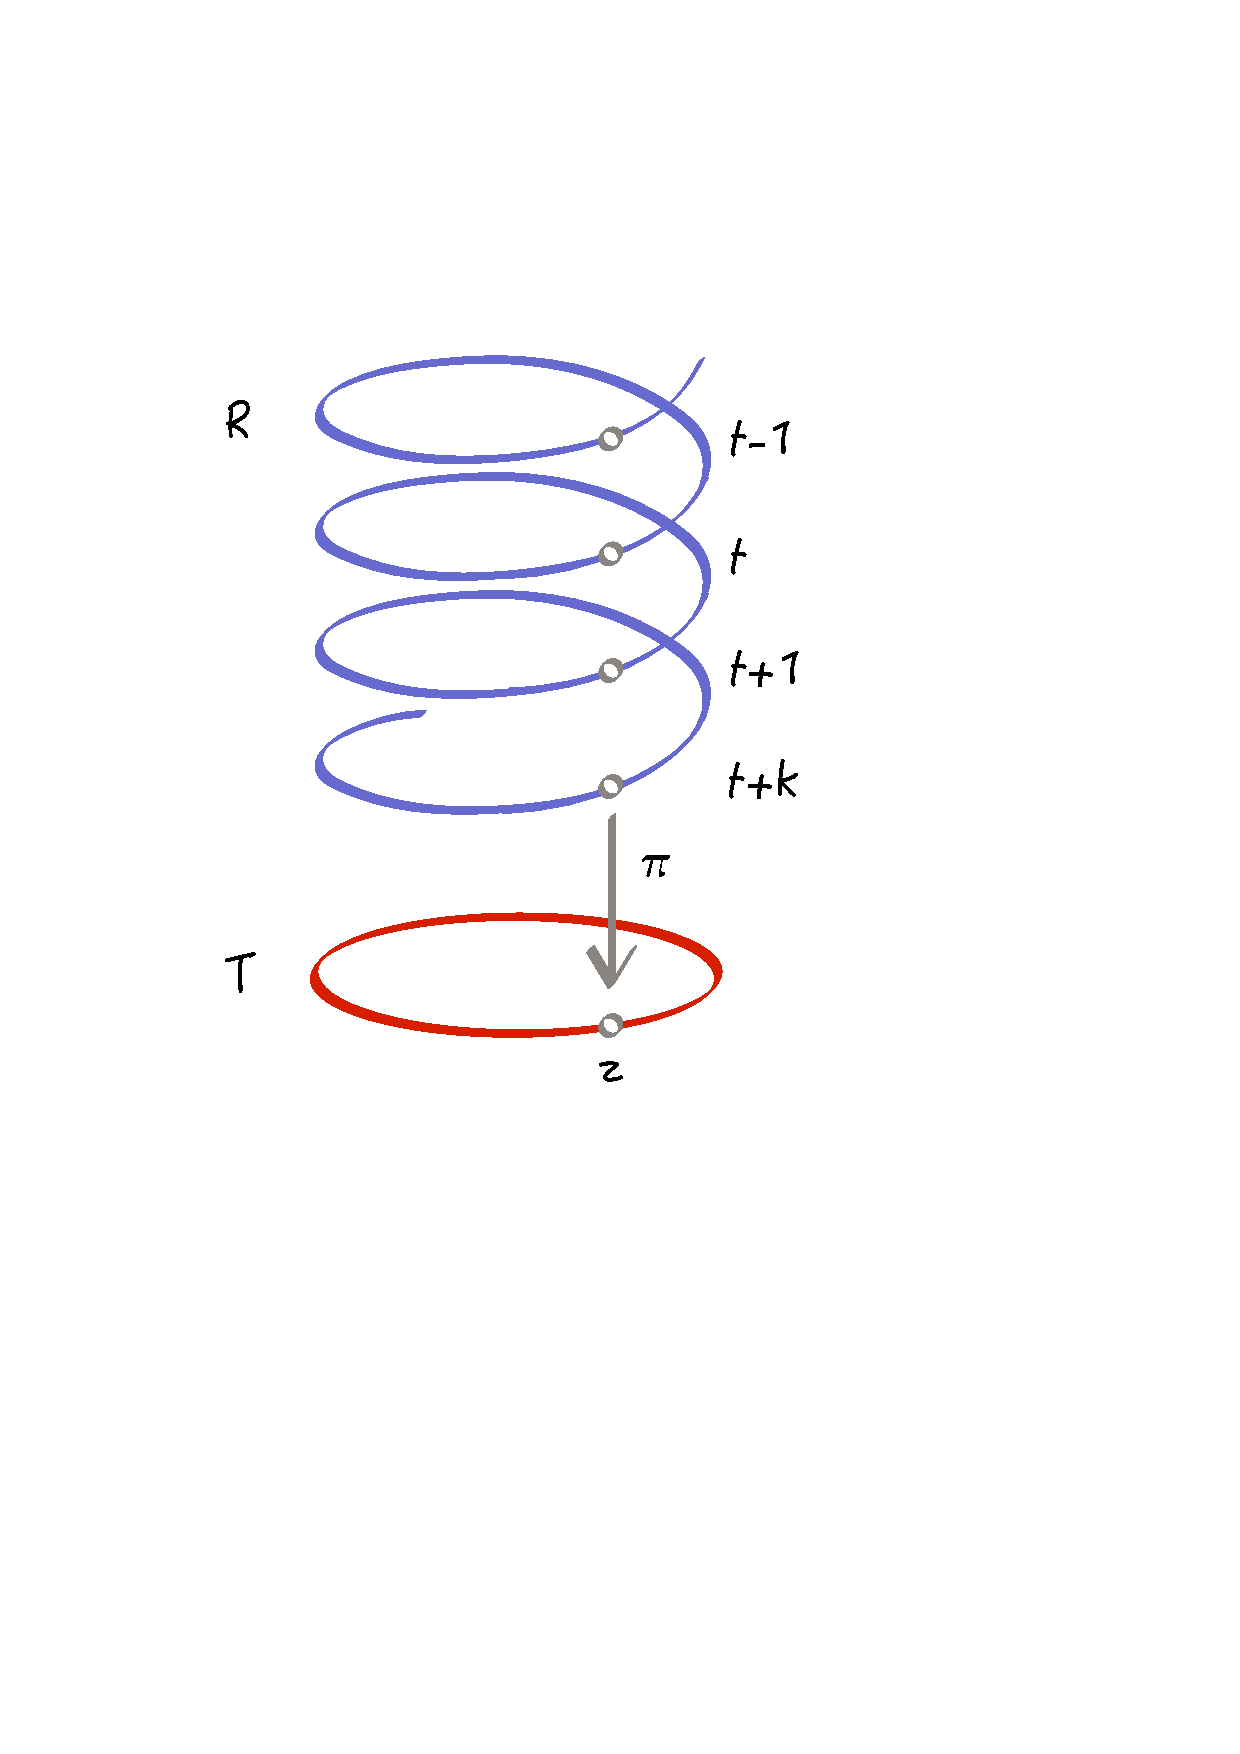
\includegraphics[width=.33\textwidth]{Figures/Covering-T.pdf}
  \caption{Covering of the Circle.}
  \label{Covering-of-the-Circle.}
\end{figure}
It is a \emph{diffeological group} (actually, a Lie group).
Moreover,
the projection $\pi$ is the \emph{universal covering} of $\Torus$,
which exists and is unique up to an isomorphism for any \emph{connected} diffeological space.
These words will be defined precisely later.

Now, the $2$-torus
$$%
  \Torus^2 = \Torus \times \Torus \subset \RR^2 \times \RR^2
  $$%
is the product of the torus $\Torus$ by itself,
its square.
It is equipped with the product diffeology we have seen in the previous lecture.
A plot of in $\Torus^2$ is a parametrization
$$%
  r \to (z_1(r),z_2(r)) = \bigg(\big(x_1(r),y_1(r)\big), \big(x_2(r),y_2(r)\big)\bigg)
  $$%
such that the $x_i$ and $y_i$ are smooth parametrizations such that $x_i(r)^2 + y_i(r)^2 = 1$ for all $r$.

Next,
we can consider the square of the projection $\pi$,
let us denote it just by $\pi_2$
$$%
  \pi_2 \colon \RR^2 \to \Torus^2
  $$%
with
$$%
  \pi_2 (t_1,t_2) = \bigg(\big(\cos(t_1),\sin(t_1)\big), \big(\cos(t_2),\sin(t_2)\big)\bigg)
  $$%
Since the projection $\pi$ on each factor is a subduction from $\RR$ onto its image $\Torus \subset \RR^2$,
the product $\pi_2$ is a subduction from $\RR^2$ onto its image $\Torus^2 \subset (\RR^2)^2$.
Therefore the square $\Torus^2$ of $\Torus$ identifies with the quotient
$$%
  \Torus^2 \simeq (\RR/\ZZ)^2 = \RR^2/\ZZ^2,
  $$%
\begin{figure}[ht]
  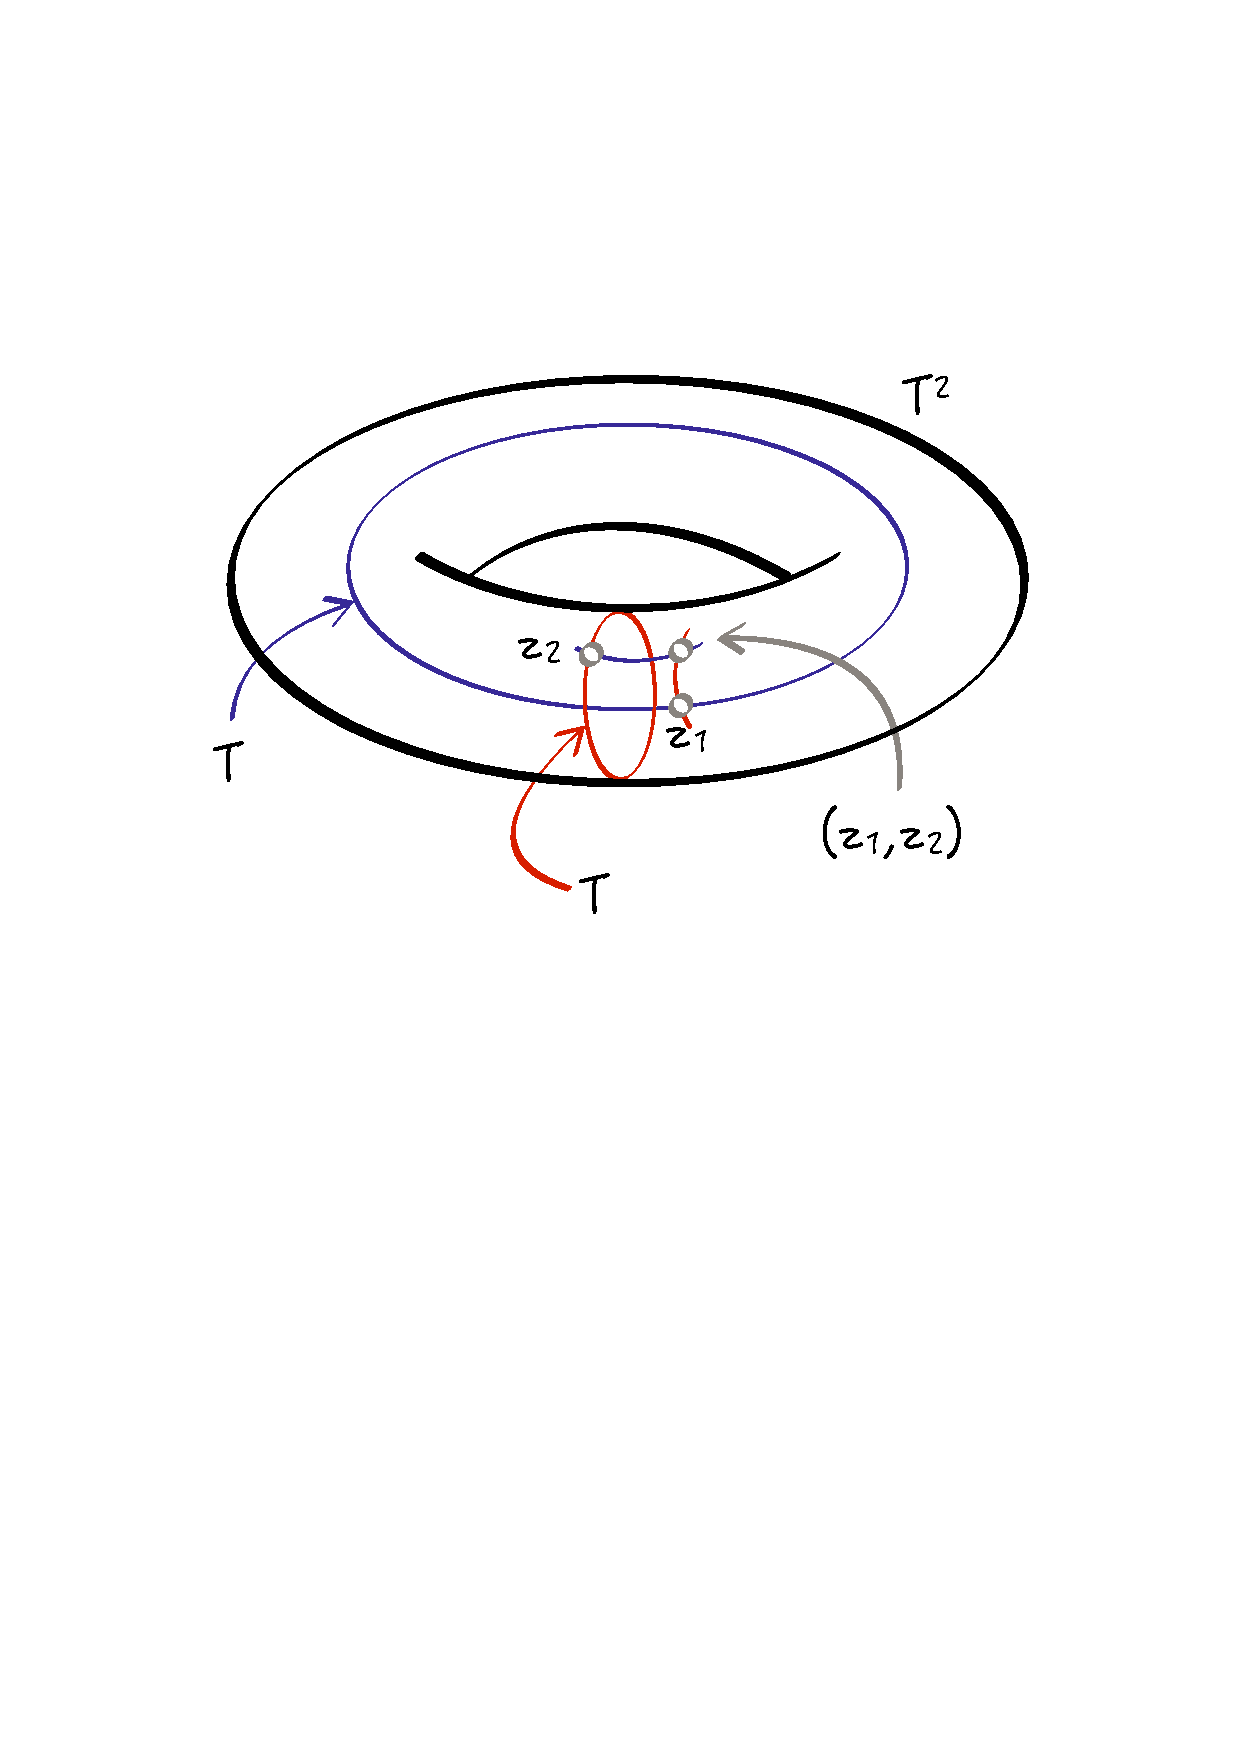
\includegraphics[width=.45\textwidth]{Figures/2-Torus.pdf}
  \caption{The $2$-torus.}
  \label{{2-Torus}}
\end{figure}
where $\ZZ^2 \subset \RR^2$ is the subset of points with integer coordinates.
More generally,
an $n$-dimensional torus $\Torus^n$ is the $n$-th power of the $1$-dimensional torus $\Torus$
$$%
  \Torus^n = \{ (z_1,\dots,z_n) \mid \forall i, z_i \in \Torus \}.
  $$%
And also equivalent to the quotient
$$%
  \Torus^n \simeq (\RR/\ZZ)^n = \RR^n/\ZZ^n.
  $$%
where $\ZZ^n \subset \RR^n$ is the subgroup of points with integer coordinates.
Again,
$\Torus^n$ is a diffeological group (a Lie group more precisely),
an Abelian one.

\uline{Remark.} Consider a \emph{lattice} in $\RR^n$,
that is,
a subgroup like
$$%
  L = \left\{ \sum_{i = 1}^n n_i v_i \mid n_i \in \ZZ \right\},
  $$%
where the $(v_i)_{i=1}^n$ are a basis of $\RR^n$.
Then the quotient space $\RR^n/L$ is naturally diffeomorphic to $\Torus^n$.
Indeed,
let $M \colon \RR^n \to \RR^n$ be the linear isomorphism $M(x) = \sum_{i=1}^n x_i v_i$,
with $x = (x_1,\dots,x_n)$.
The map
$$%
  m = \Class(x) \mapsto \Class_L(x)
  $$%
is well defined and defines a smooth group isomorphism from $\Torus^n = \RR^n/\ZZ^n$ to $\RR^n/L$.
\begin{center}
  \begin{tikzcd}[column sep=small, row sep=large, every label/.append style = {font = \small}]
    & \RR^n \arrow[dl, swap, "\Class"] \arrow[dr, "\Class_L"] &          \\
    \RR^n/\ZZ^n \arrow[rr, swap, "m"] &                                                          & \RR^n/L
  \end{tikzcd}
\end{center}
So,
diffeologically speaking there is only one torus $\Torus^n$:
all lattices are equivalent.

The various tori are often described as the power of the unitary group
$$%
  \U(1) = \{ z \in \CC \mid \bar z z = 1 \},
  $$%
where $\bar z$ denotes $z$ conjugate.
Thus,
$$%
  \Torus^n \simeq \U(1)^n = \{ (z_1,\dots,z_n) \mid \forall i, z_i \in \U(1) \}
  $$%
There,
the group law is just the pointwise multiplication:
$$%
  (z_1,\dots,z_n) \cdot (z'_1,\dots,z'_n) = (z_1z'_1,\dots,z_nz'_n).
  $$%
We remark that the multiplication is smooth,
that means that for two plots $r \mapsto (z_1(r),\dots,z_n(r))$ and $r \mapsto (z'_1(r),\dots,z'_n(r))$,
defined on the same domain,
the resulting parametrization $r \mapsto (z_1(r)z'_1(r),\dots,$%
\linebreak
$z_n(r)z'_n(r))$ is again a plot in $\Torus^n$.
The inversion $r \mapsto (\bar z_1(r),\dots,\bar z_n(r))$ also is smooth.
We say that $\Torus^n$ is a \emph{diffeological group}.
We shall develop later a little bit about diffeological groups,
especially when it will come to the moment map and symplectic diffeology.
But for now,
that is all we need.

%%%%%%%%%%%%%%%%%%%%%%%%%%%%%%%%%%%%%%%%%%%%%%%%%%%%%%%%%%
%%
%% MARK: The Irrational Torus $\Torus_\alpha$
%%
%%%%%%%%%%%%%%%%%%%%%%%%%%%%%%%%%%%%%%%%%%%%%%%%%%%%%%%%%%

\section{The irrational torus $\Torus_\alpha$}

The object ``irrational torus'' has been motivated by physics,
by a question related to the behavior of a particle submitted to a quasiperiodic potential.
These quasiperiodic potentials describe the phenomenon of a quasiperiodic pattern in crystals.
For example,
Figure \ref{A-Quasicristal} is representing the diffraction of an aluminium-palladium-manganese (Al-Pd-Mn) quasicrystal surface.
\begin{figure}[ht]
  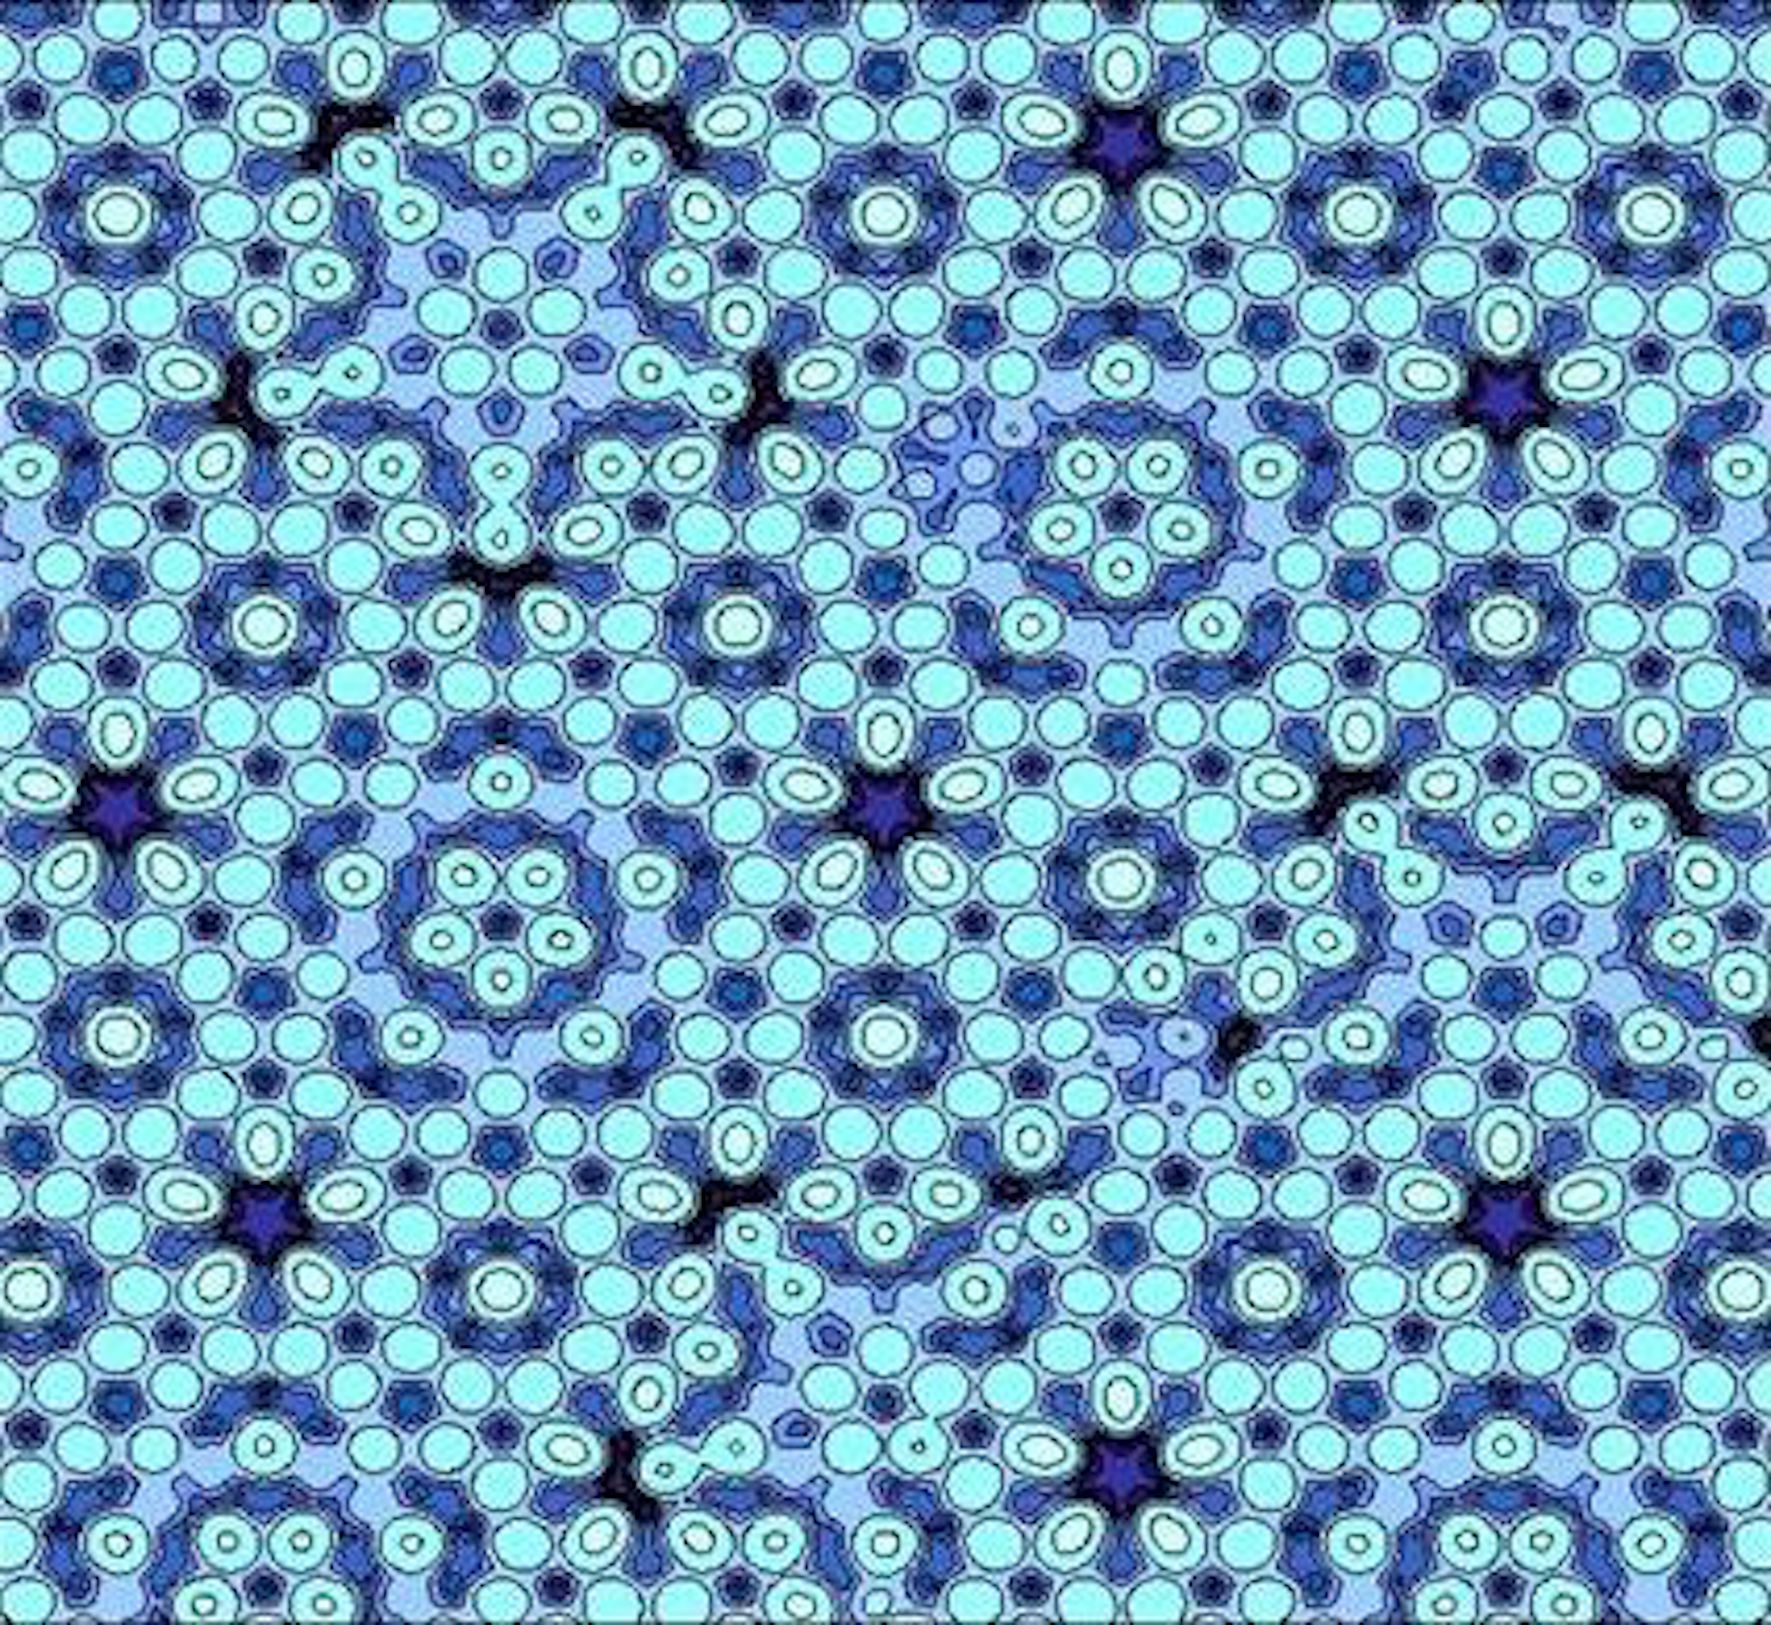
\includegraphics[width=.45\textwidth]{Figures/Quasicrystal.jpg}
  \caption{A Diffraction Figure of a Quasicrystal.}
  \label{A-Quasicristal}
\end{figure}
For this type of material,
the diffraction pattern is not periodic as it is usually for a crystal,
i.e. it does not draw a periodic tiling of the plane,
but something close without being quite so.

The physicists and the mathematicians who were involved in this research decided that,
that phenomenon could be described by a \emph{quasiperiodic potential}.
I will try to outline their approach without being able to be too precise.

In classical physics,
the motion of a particle in a medium is described by a force which is the gradient of a real function called the \uline{potential}.

So,
let us consider the simplest example,
a toy model:
a particle moving on a line submitted to a force that is the derivative of a real function $V : \RR \to \RR$,
which is assumed to be smooth.
Physicists are interested in the spectrum of the so-called (quantum) Hamiltonian:
$$%
  \hat H = -{\hbar \over 2m} {\partial^2 \over \partial x^2} + V(x)
  $$%
which is an operator on some Hilbert space of functions.
Two main special cases are illustrated by Figure \ref{P-QP-Potential}.

\begin{enumerate}
  \item The \emph{periodic case} is described by the potential
  $$%
    V_1 \colon x \mapsto U_1\left(e^{2i\pi x}\right)
    $$%
  where $U_1$ is defined on the circle $\Sph^1$.
  \item The \emph{quasiperiodic case} is described by the potential
  $$%
    V_2 \colon x \mapsto U_2 \circ j_\alpha(x),
    $$%
  where $U_2$ is a function defined on the $2$-torus and $j_\alpha \colon \RR \to \Torus^2$ is the map
  $$%
    j_\alpha \colon x \mapsto \left(e^{2i\pi x}, e^{2i\pi\alpha x}\right)
    \quad \text{with} \quad
    \alpha \in \RR - \QQ.
    $$%
\end{enumerate}

\begin{figure}[ht]
  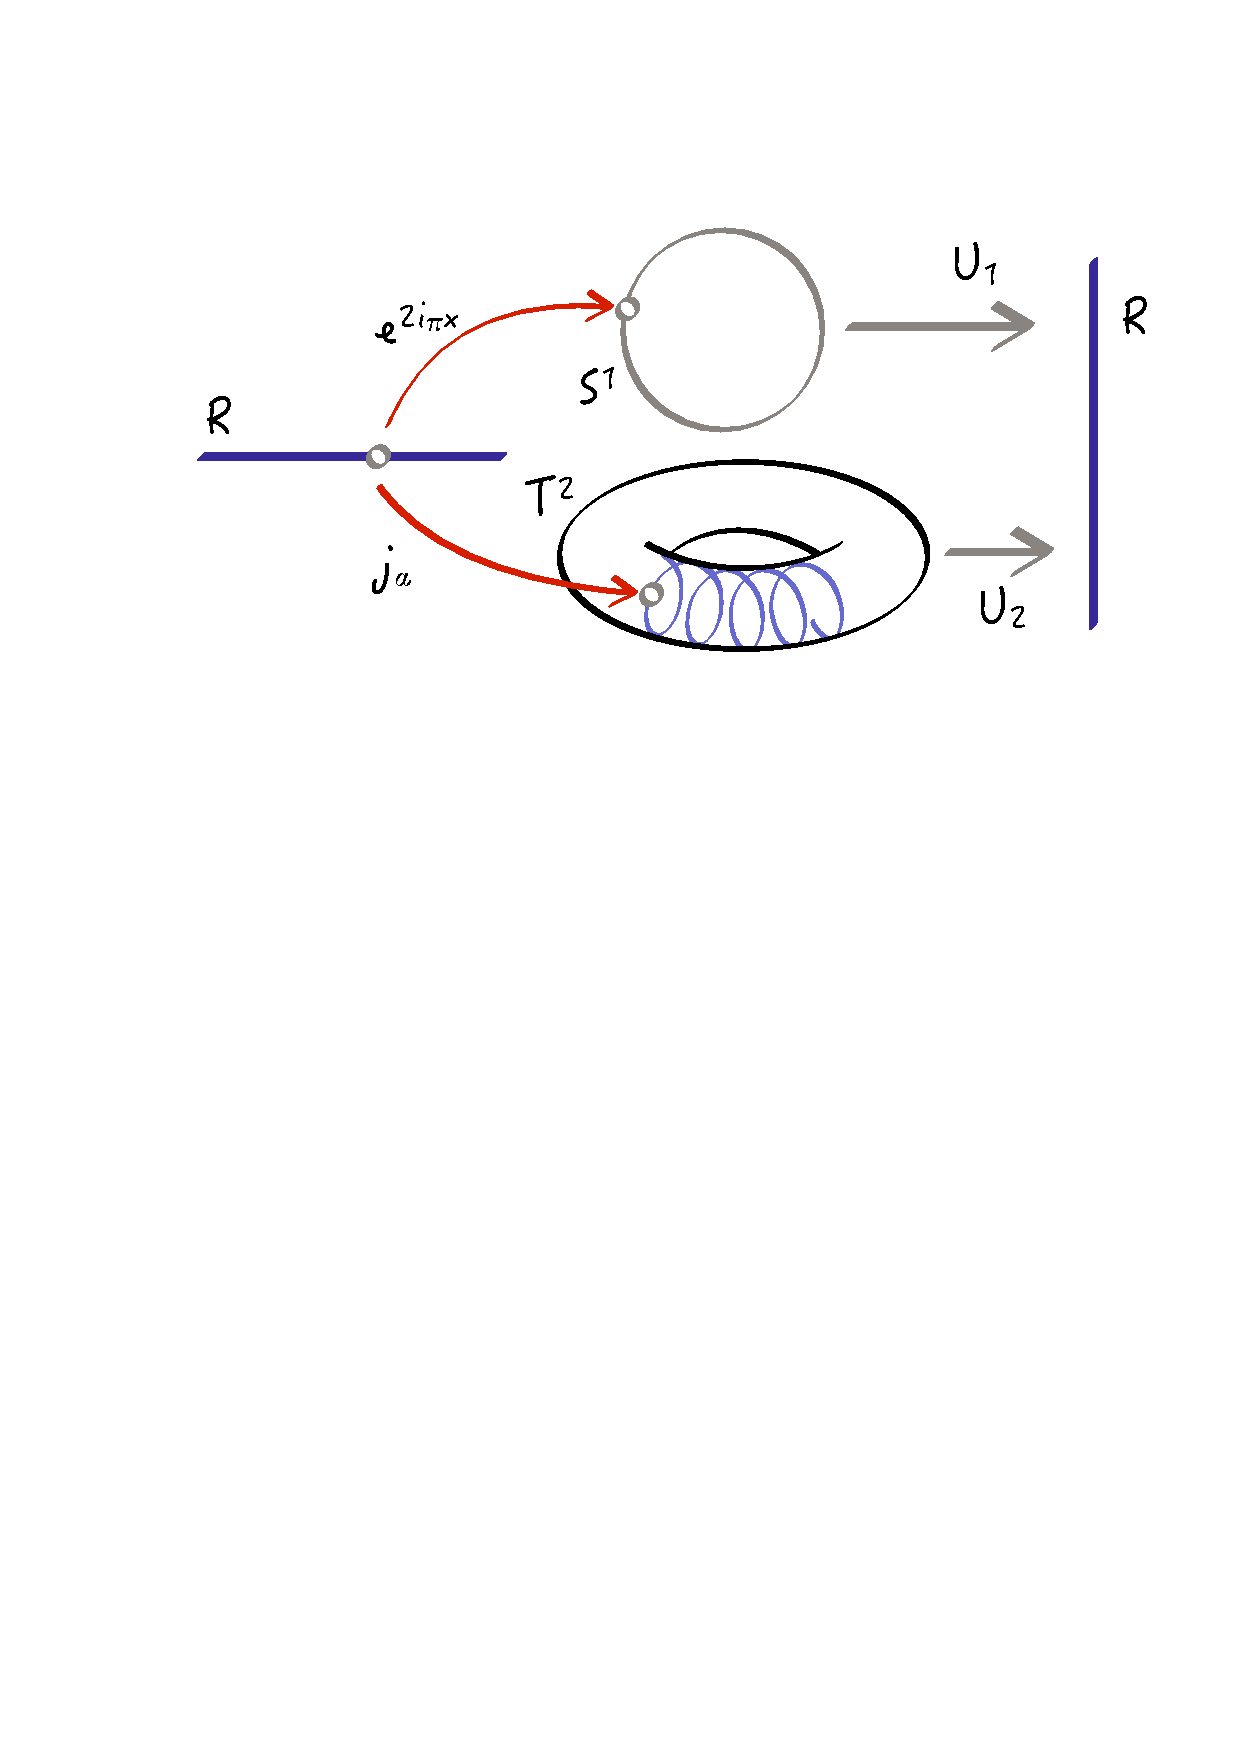
\includegraphics[width=0.70\textwidth]{Figures/P-QP-Potential.pdf}
  \caption{Periodic and Quasiperiodic Potential.}
  \label{P-QP-Potential}
\end{figure}

So,
the quasiperiodic property is encoded in the \emph{irrational solenoid}
$$%
  \cS_\alpha = \left\{ \left(e^{2i\pi x}, e^{2i\pi\alpha x}\right) \mid x \in \RR \right\}.
  $$%
We remark first that $\cS \subset \Torus^2$ is a subgroup.

Our intention now is not to solve the general question of the spectrum of the Hamiltonian in presence of quasiperiodic potential,
but to delve deeper into issues surrounding these contexts.
In particular:

\begin{Article}{Definition.}{\itshape}
  We call \emph{irrational torus $\Torus_\alpha$} the quotient space
  $$%
    \Torus_\alpha = \Torus^2/\cS_\alpha,
    $$%
  equipped with the quotient diffeology.
\end{Article}

\begin{Article}{Proposition.}{}
  The map $j_\alpha \colon x \mapsto \left(e^{2i\pi x}, e^{2i\pi\alpha x}\right)$ is an induction from $\RR$ into $\Torus^2$,
  with image the solenoid $\cS_\alpha$.
  
  \Note We shall see further on,
  $\cS_\alpha \subset \Torus^2$ is a submanifold in the sense of diffeological manifolds,
  but not exactly in the usual sense because it is not embedded.
  In ordinary differential geometry textbooks,
  submanifolds are defined only embedded.
\end{Article}

\begin{proof}
  We begin to check that the map $\pi^2 : (x,y) \mapsto (\pi(x), \pi(y))$, where
  $\pi(t) = (\cos(2\pi t),\sin(2\pi t))$, from $\RR \times \RR$ to $\RR^2 \times \RR^2$ is strict.
  First of all,
  the map $\pi^2$ is smooth.
  Then,
  according to the definition, $\pi^2$ is strict if and only if
  $$%
    \Class(x,y) \mapsto \left(\big(\cos(2\pi x),\sin(2\pi x)\big),\big(\cos(2\pi y),\sin(2\pi y)\big)\right)
    $$%
  is an induction, from $\RR^2/\ZZ^2$ to $\RR^2 \times \RR^2$,
  with $\Class : \RR^2 \to \RR^2/\ZZ^2$.
  We have already seen that $\pi : t \mapsto (\cos(2\pi t),\sin(2\pi t))$ is strict,
  and $\pi^2$ is just the square of $\pi$.
  Thus,
  a plot $\Phi : U \to \Sph^1 \times \Sph^1 \subset \RR^2 \times \RR^2$ is just a pair of plots $P$ and $Q$ from $U$ to $\Sph^1$,
  which can be individually smoothly lifted locally along $\pi$,
  and give a local lift of $\pi^2$ itself.
  Thus, $\pi^2$ is strict.
  
  Now,
  let $\Delta_\alpha$ be the line in $\RR \times \RR$ with slope $\alpha$,
  the subset of points $(x,\alpha x) \in \RR^2$.
  Since
  $\alpha$ is irrational, $\pi^2_\alpha = \pi^2 \restriction \Delta_\alpha$ is injective.
  Indeed,
  $\pi^2(t,\alpha t) = \pi^2(t',\alpha t')$ means,
  on the one hand,
  $(\cos(2\pi t'),\sin(2\pi t')) = (\cos(2\pi t),\sin(2\pi t))$,
  and on the other hand,
  $(\cos(2\pi \alpha t'),\sin(2\pi \alpha t')) = (\cos(2\pi \alpha t),\sin(2\pi \alpha t))$.
  That is,
  $t' = t + k$ and $\alpha t' = \alpha t + k'$ with $k,k' \in \ZZ$,
  which gives $\alpha k - k' = 0$,
  but $\alpha \notin \QQ$,
  thus $k = k' = 0$ and then $t'=t$.
  
  Let
  $\Phi : U \to \cS_\alpha \subset \Sph^1 \times \Sph^1 \subset \RR^2 \times \RR^2$ be a
  plot, with $\Phi(r)=(P(r),Q(r))$. Since $\pi^2$ is strict, for all $r \in U$,
  there exists locally a smooth lift $r' \mapsto (x(r'),y(r'))$ in $\RR^2$,
  defined on a neighborhood $V$ of $r$, such that $\pi^2(x(r'),y(r')) = (P(r'),Q(r'))$
  Thus, $\pi^2(x(r'),y(r')) \in \cS_\alpha$
  for all $r' \in V$. But,
  $r' \mapsto (x(r'),\alpha x(r')) \in \Delta_\alpha \subset \RR^2$ is smooth,
  and $\pi^2(x(r'),\alpha x(r'))$ belongs to $\cS_\alpha$ too.
  Therefore, there exists $r' \mapsto k(r') \in \ZZ$ such that
  $y(r') = \alpha x(r') + k(r')$, that is,
  $k(r') = y(r') - x(r')$.
  Thus, $r' \mapsto k(r')$ is smooth and takes its values in $\ZZ$, hence
  $k(r') = k$ constant. Then,
  $r' \mapsto (x(r'), y(r') - k)$ is a plot of $\cS_\alpha$
  with $\pi^2(x(r'), y(r') - k) = (P(r'),Q(r'))$, thus
  $\pi^2_\alpha : \Delta_\alpha \to \cS_\alpha$ is an injective subduction,
  that is, a diffeomorphism from $\Delta_\alpha$
  to $\cS_\alpha$, and therefore an induction.
\end{proof}

\begin{Article}{Proposition.}{}
  The quotient space $\Torus_\alpha = \Torus^2/\cS_\alpha$ is diffeomorphic to the quotient $\RR/(\ZZ + \alpha \ZZ)$,
  and isomorphic as a group.
  
  \Note{1.} It is clear now that $\Torus_\alpha$,
  as a quotient topological space,
  is trivial since $\ZZ + \alpha \ZZ \subset \RR$ is dense.
  
  \Note{2.} $\Torus_\alpha$ is also isomorphic to the intermediate quotient $\RR^2 / \ZZ^2(\Delta_\alpha)$,
  where $\ZZ^2(\Delta_\alpha)$ is the image of the line $\Delta_\alpha$ by $\ZZ^2$,
  that is,
  the set of points $(x+n, \alpha x + m)$ with $x \in \RR$ and $(n,m) \in \ZZ^2$.
\end{Article}

\begin{proof}
  We begin to prove that with $\alpha \notin \QQ$,
  $\ZZ + \alpha \ZZ$ is dense in $\RR$.
  We remark first that $\ZZ + \alpha \ZZ$ is a subgroup of $(\RR,+)$.
  Let $\Gamma \subset \RR$ be a subgroup not reduced to $\{0\}$.
  It is relatively obvious that:
  either there exists a smallest element $a \in \Gamma$ and $\Gamma = a \ZZ$,
  or $\Gamma$ is dense.
  Now,
  if $\ZZ + \alpha \ZZ = a \ZZ$,
  then $\alpha = ka$ and $1 = \ell a$ with $k,\ell \in \ZZ$,
  that would mean that $\alpha = k/\ell$ which is not the case.
  Thus,
  $\ZZ + \alpha \ZZ$ is dense.
  
  Let $\pphi \colon \RR^2/\ZZ^2 \to \Sph^1 \times \Sph^1$ be the identification given by the factorization of the strict map $\pi^2 \colon \RR^2 \to \Sph^1 \times \Sph^1$.
  Then,
  the quotient $(\Sph^1 \times \Sph^1)/\cS_\alpha = \pphi(\RR^2/\ZZ^2)/\cS_\alpha$,
  is equivalent to $\RR^2/[\ZZ^2(\Delta_\alpha)]$ where the equivalence relation is
  defined by the action of the subgroup $\ZZ^2(\Delta_\alpha)$.
  Let $\rho : \RR^2 \to \RR^2$ be defined
  by $\rho(x,y) = (0, y -\alpha x)$,
  it is obviously a projector,
  $\rho \circ \rho = \rho$,
  and clearly $\Class \circ\,\rho = \Class$,
  with $\Class : \RR^2 \to \RR^2/[\ZZ^2(\Delta_\alpha)]$.
  \begin{figure}[ht]
    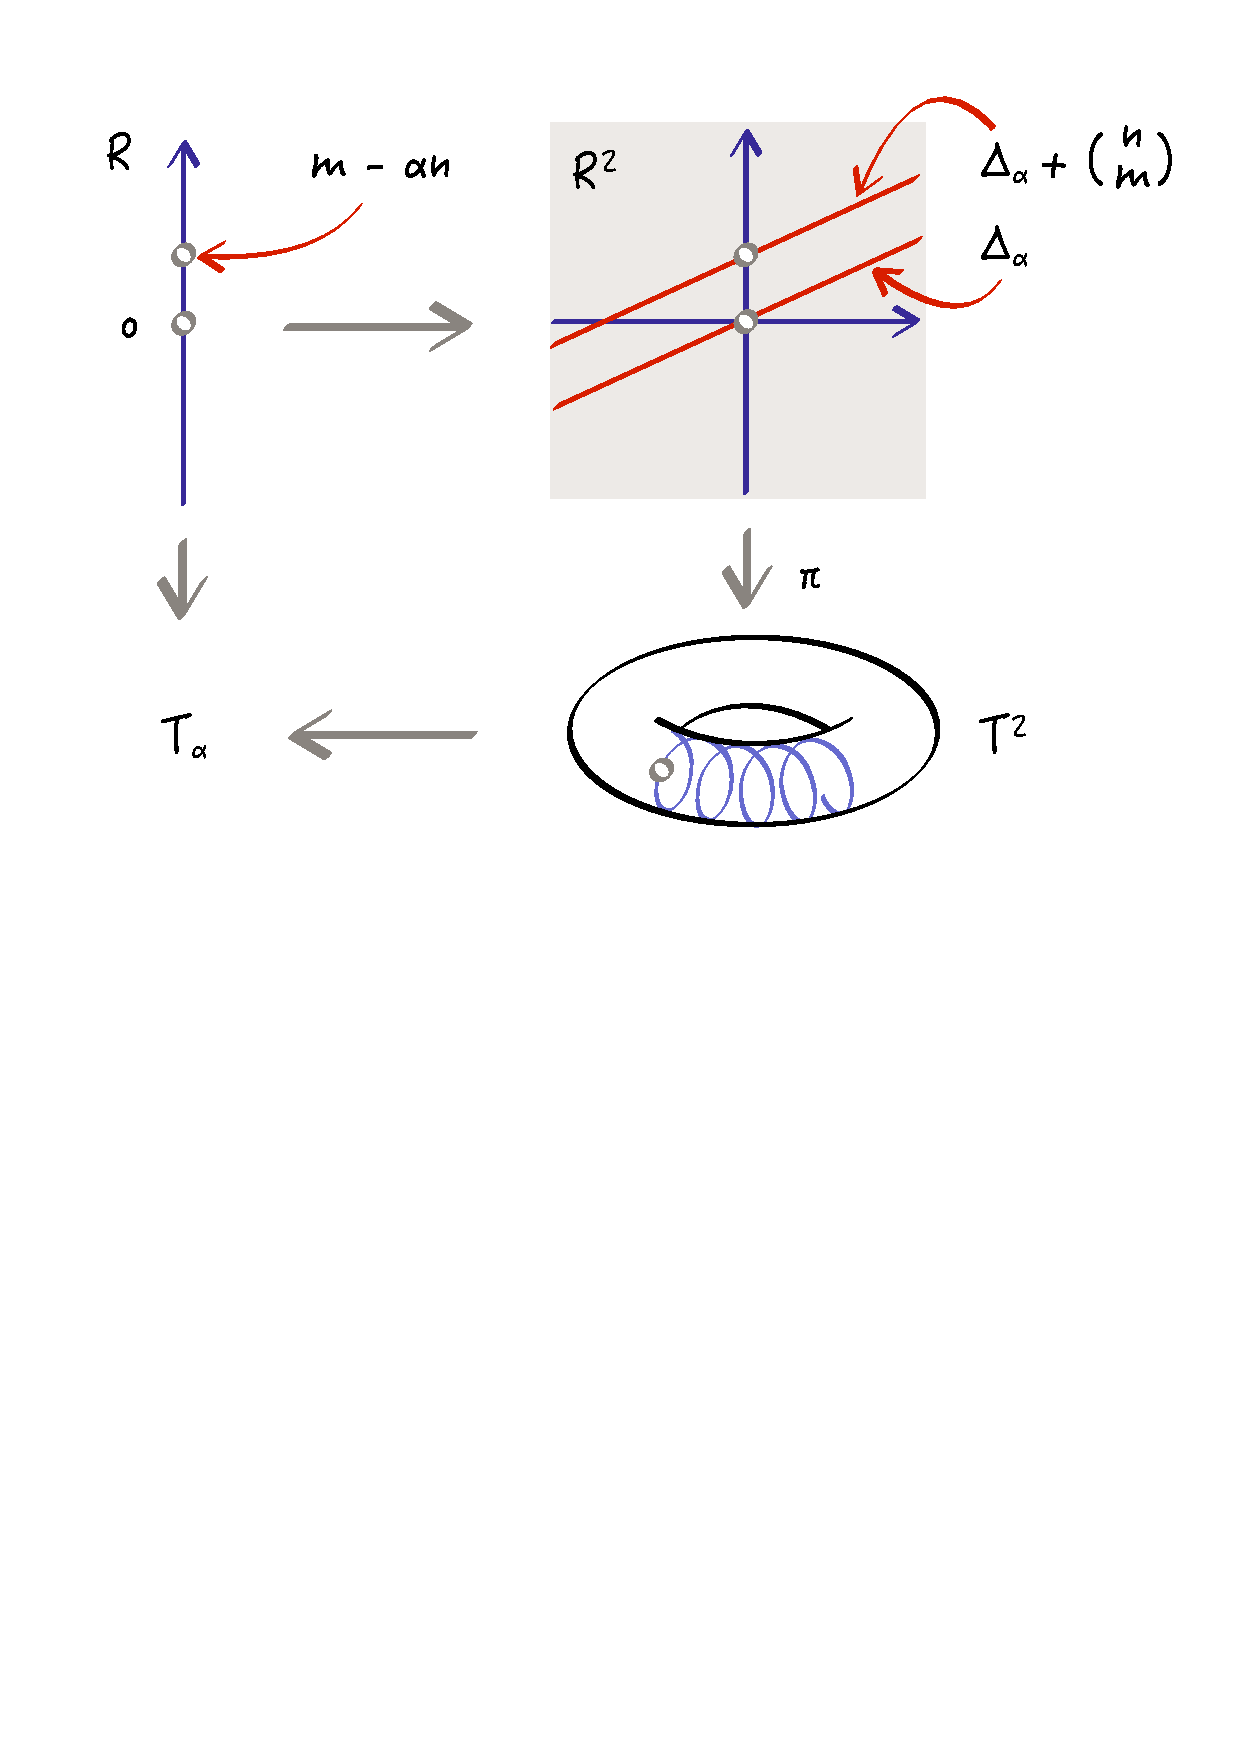
\includegraphics[width=0.75\textwidth]{Figures/Ta-Quotient.pdf}
    \caption{$\Torus_\alpha$ as quotients.}
    \label{Ta-Quotient}
  \end{figure}
  Now,
  let $X' = \Val(\rho)$, that is, $X' = \{0\} \times \RR$.
  The restriction to $X'$ of the equivalence relation defined by the action of $\ZZ^2(\Delta_\alpha)$ on $\RR^2$,
  is given by the following action of $\ZZ^2$,
  $(n,m) \colon (0,y) \mapsto (0, y + m -\alpha n)$. Therefore, the quotient
  $(\Sph^1 \times \Sph^1)/\cS_\alpha$ is equivalent to $X'/(\ZZ + \alpha \ZZ)$,
  that is, equivalent to $\RR/(\ZZ + \alpha \ZZ) = \Torus_\alpha$.
\end{proof}

\begin{Article}{Smooth maps from $\Torus_\alpha$ to $\Torus_\beta$.}{}
  For any pair $\alpha$ and $\beta$ of irrational numbers,
  the set $\Cinfty(\Torus_\alpha,\Torus_\beta)$ does not reduce to the constant maps if and only if there exists  $a,b,c,d \in \ZZ$ such that
  $$%
    \alpha = {c + d \beta \over a + b \beta}.
    $$%
  Note that,
  since $\alpha$ and $\beta$ are irrational,
  the relation above has an inverse $\beta = (a \alpha - c) / (d - b \alpha)$.
\end{Article}

\begin{proof}
  Let $f \colon \Torus_\alpha \to \Torus_\beta$ be a smooth map.
  Consider the commutative diagram
  \begin{center}
    \begin{tikzcd}[column sep=large, row sep=large, every label/.append style = {font = \small}]
      \RR \arrow[r, dashed, "F"] \arrow[d, swap, "\Class_\alpha"] &  \RR  \arrow[d, "\Class_\beta"]  \\
      \Torus_\alpha \arrow[r, swap, "f"] & \Torus_\beta
    \end{tikzcd}
  \end{center}
  Since $\Class_\alpha$ is a plot in $\Torus_\alpha$,
  $f \circ \Class_\alpha$ is a plot of $\Torus_\beta$.
  Hence,
  for every real $x_0$ there exists an open interval $V$ centered at $x_0$,
  and a smooth parametrization $F : V \to \RR$ such that $\Class_\beta \circ F = (f \circ \Class_\alpha) \restriction V$.
  For all real numbers $x$ and all pairs $(n,m)$ of integers such that $x + n + \alpha m \in V$,
  there exist two integers $n'$ and $m'$ such that
  \begin{equation} \tag{$\spadesuit$}
    F(x + n + \alpha m) = F(x) + n' + \beta m'.
  \end{equation}
  Since $\beta$ is irrational, for every such $x$, $n$ and $m$,
  \uline{the pair $(n',m')$ is unique}.
  
  Now,
  there exists an interval $\cJ \subset V$ centered at $x_0$ and an interval $\cO$ centered at $0$ such that:
  for every $x \in \cJ$ and for every $n + \alpha m \in \cO$,
  $x + n + \alpha m \in V$.
  \begin{figure}[ht]
    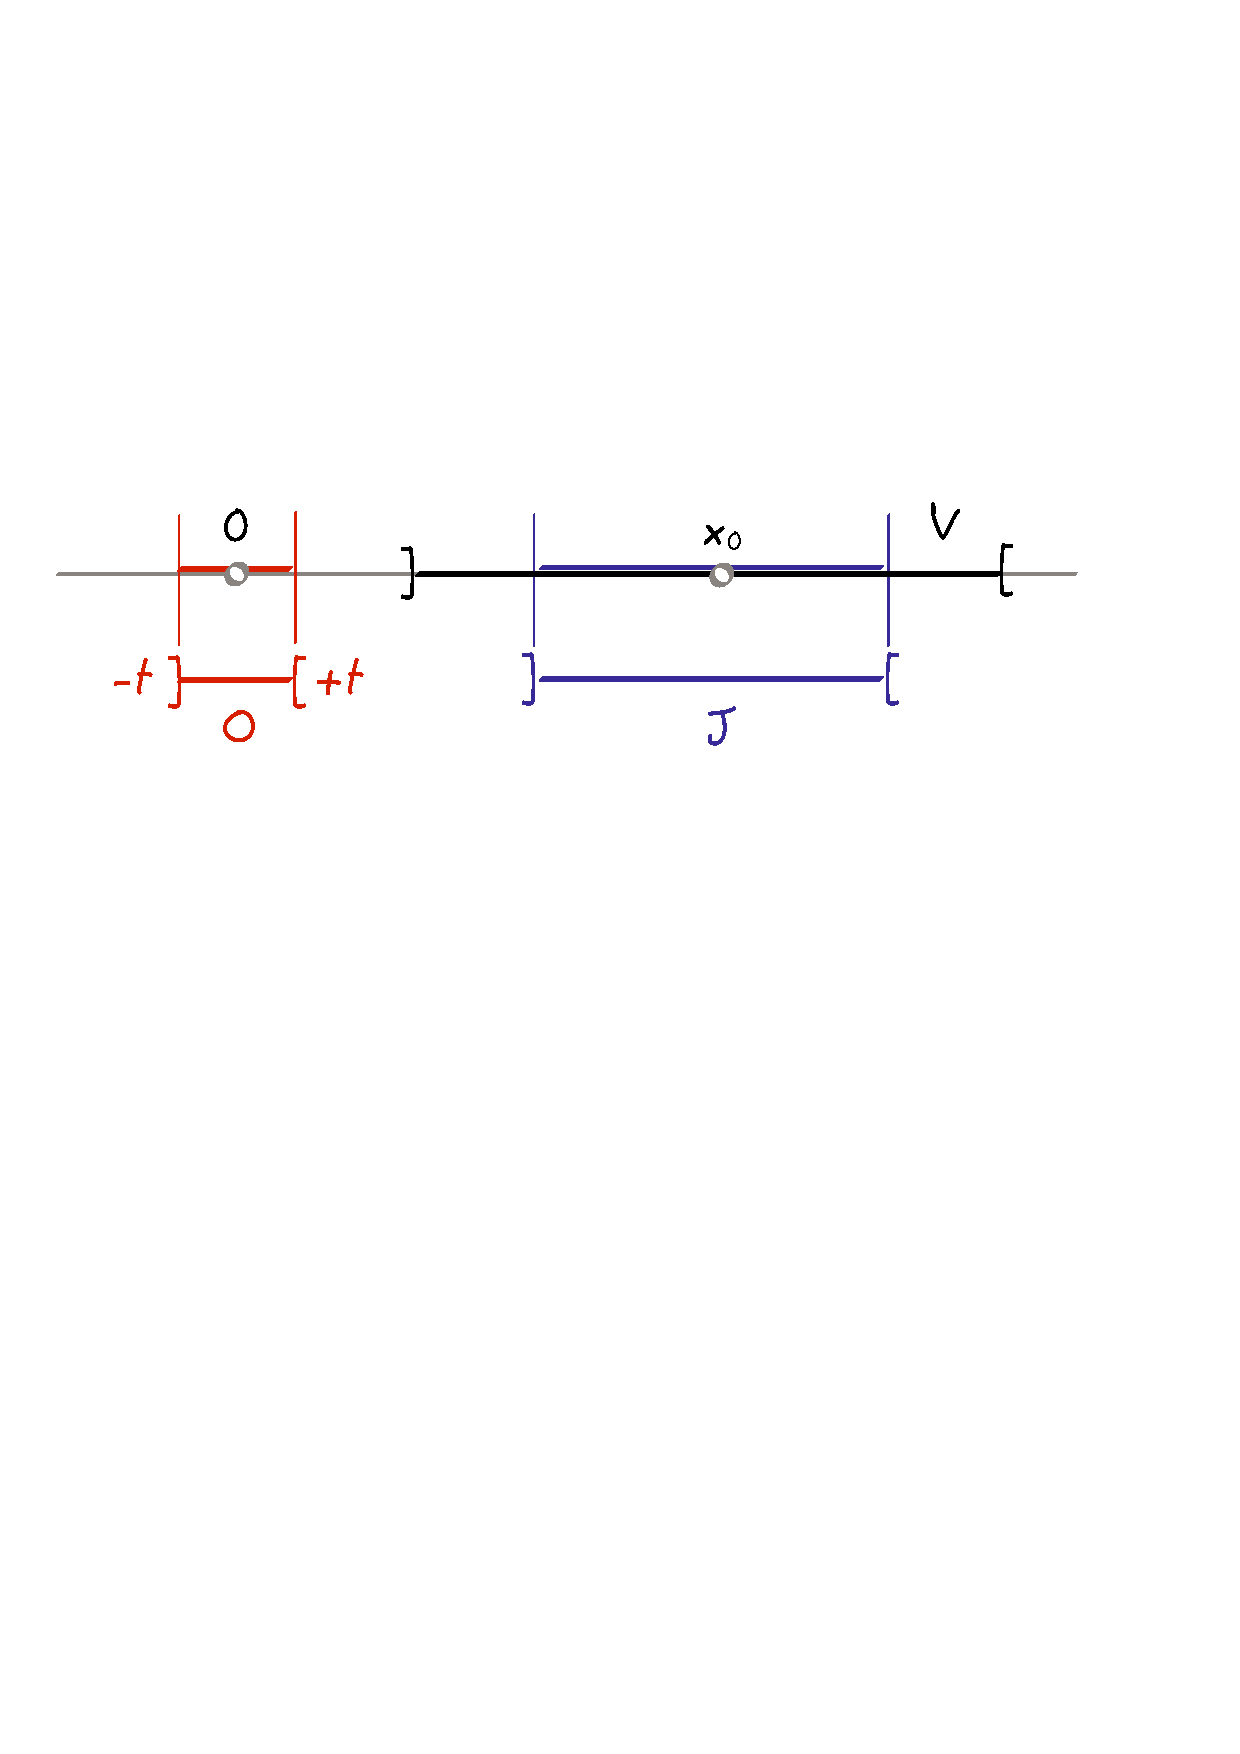
\includegraphics[width=0.66\textwidth]{Figures/OJ-Intervals.pdf}
    \caption{Intervals $V,\cO, J$.}
    \label{OJ-Intervals}
  \end{figure}
  Since $F$ is continuous and since $\ZZ + \alpha \ZZ$ is diffeologically discrete,
  $n' + \beta m' = F(x + n + \alpha m) - F(x)$ is constant as function of $x$.
  But $F$ is smooth,
  the derivative of the identity ($\spadesuit$),
  with respect to $x$,
  at the point $x_0$,
  gives $F'(x_0 + n + \alpha m) = F'(x_0)$.
  Then,
  since $\alpha$ is irrational,
  $\ZZ + \alpha \ZZ \cap \cO$ is dense in $\cO$,
  and since $F'$ is continuous,
  $F'(x) = F'(x_0)$,
  for all $x \in \cJ$.
  Hence,
  $F$ restricted to $\cJ$ is affine,
  there exist two numbers $\lambda$ and $\mu$ such that
  \begin{equation} \tag{$\clubsuit$}
    F(x) = \lambda x + \mu \quad \text{for all} \quad x \in \cJ.
  \end{equation}
  Note that,
  by density of $\ZZ + \alpha \ZZ$,
  $\Class_\alpha(\cJ) = \Torus_\alpha$.
  Hence \uline{$F$ defines completely the function $f$}.
  
  Now, applying ($\spadesuit$) to the expression ($\clubsuit$) of $F$,
  we get for all $n + \alpha m \in \cO$:
  $\lambda(x + n + \alpha m) + \mu = \lambda x + \mu  + n' + \beta m'$,
  that is:
  \begin{equation} \tag{$\diamondsuit$}
    \lambda \times (n + \alpha m ) \in \ZZ + \beta \ZZ,
    \quad \text{that is:} \quad
    \lambda (\ZZ + \alpha \ZZ) \subset \ZZ + \beta \ZZ.
  \end{equation}
  Let us show that \uline{actually $(\diamondsuit)$ is satisfied for all $n + \alpha m$ in $\ZZ + \alpha \ZZ$}.
  Let $\cO = \OpenInterval{-t,t}$,
  and let us take $t$ not in $\ZZ + \alpha \ZZ$,
  even if we have to shorten $\cO$ a little.
  Let $x \in \ZZ + \alpha \ZZ$,
  and $x >t$.
  There exists $N \in \NN$ such that
  $$%
    0 < (N-1)t < x < N t,
    \quad \text{and then} \quad
    0< {x \over N} < t.
    $$%
  Now, by density of $\ZZ + \alpha \ZZ$ in $\RR$,
  $$%
    \forall  \eta >0, \quad \exists y > 0 \quad \text{such that} \quad y \in \ZZ + \alpha \ZZ \quad \text{and} \quad 0 < {x \over N} - y < \eta.
    $$%
  Choosing $\eta < t/N$ we have
  $$%
    \eta < {t \over N} \quad \Rightarrow \quad 0 < x - N y < N \eta < t
    \quad \text{and} \quad
    0 < y < {x \over N} < t.
    $$%
  Hence,
  $$%
    x, y \in \ZZ + \alpha \ZZ \quad \Rightarrow \quad x-Ny \in \ZZ + \alpha \ZZ,
    $$%
  and
  $$%
    x - N y < t \quad \Rightarrow \quad x - N y \in \ZZ + \alpha \ZZ \cap \cO.
    $$%
  Thus,
  $$%
    \lambda \times (x- N y) = \lambda x - N \times (\lambda y) \in \ZZ + \beta \ZZ.
    $$%
  But,
  $$%
    y \in  \ZZ + \alpha \ZZ \cap \cO \quad \Rightarrow \quad \lambda y \in \ZZ + \beta \ZZ \quad \Rightarrow \quad N \times (\lambda y) \in \ZZ + \beta \ZZ,
    $$%
  therefore,
  $\lambda x - N \times (\lambda y) \in \ZZ + \beta \ZZ$,
  together with $N \times (\lambda y) \in \ZZ + \beta \ZZ$,
  implies
  $$%
    \forall x \in \ZZ + \alpha \ZZ, \quad \lambda x \in \ZZ + \beta \ZZ.
    $$%
  Now, applying successively $(\diamondsuit)$ to $x = 1$ and $x = \alpha$,
  we get
  $$%
    \lambda \in \ZZ + \beta \ZZ
    \quad \text{and} \quad
    \lambda \alpha \in \ZZ + \beta \ZZ
    $$%
  Let
  $$%
    \lambda = a + b \beta.
    \quad \text{and} \quad
    \lambda \alpha = c + d \beta.
    $$%
  If $\lambda \neq 0$,
  then
  $$%
    \alpha = {c + d \beta \over a + b \beta}.
    $$%
  Let us remark that,
  since $\Class_\alpha(\cJ) = \Torus_\alpha$,
  the map $F$,
  extended to the whole $\RR$,
  still satisfies $\Class_\beta \circ F = f \circ \Class_\alpha$.
\end{proof}

\begin{Article}{Diffeomorphisms between $\Torus_\alpha$ and $\Torus_\beta$.}{}
  Let $\alpha$ and $\beta$ be two irrational numbers.
  The tori $\Torus_\alpha$ and $\Torus_\beta$ are diffeomorphic if and only if there exists  $a,b,c,d \in \ZZ$ such that
  $$%
    \alpha = {c + d \beta \over a + b \beta}
    \quad \text{with} \quad
    ad-bc = \pm 1.
    $$%
  We say $\alpha$ and $\beta$ are conjugated modulo $\GL(2,\ZZ)$ \cite{DI83}.
\end{Article}

\begin{proof}
  The map $f$ being surjective is equivalent to $\lambda \neq 0$.
  Let us express that $f$ is injective:
  let $\tau = \Class_\alpha(x)$ and  $\tau' = \Class_\alpha(x')$.
  The map $f$ is injective if  $f(\tau) = f(\tau')$ implies $\tau = \tau'$,
  that is,
  $x' = x + n + \alpha m$,
  for some relative integers $n$ and $m$.
  Using the lifting $F$,
  this is equivalent to:
  %
  \begin{itemize}
    \item[]  If there exist two integers $n'$ and $m'$ such that $F(x') = F(x) + n' + \beta m'$,
    then there exist two integers $n$ and $m$ such that $x' = x + n + \alpha m$.
  \end{itemize}
  %
  But $F(x) = \lambda x + \mu$,
  with $\lambda \times (\ZZ + \alpha \ZZ) \subset \ZZ + \beta \ZZ$.
  Hence,
  the injectivity writes:
  %
  \begin{itemize}
    \item[] If $\lambda x' + \mu = \lambda x + \mu + n' + \beta m'$,
    then $x' = x + n + \alpha m$.
  \end{itemize}
  %
  Which is equivalent to:
  %
  \begin{itemize}
    \item[] If $\lambda y \in \ZZ + \beta \ZZ$,
    then $y \in \ZZ + \alpha \ZZ$.
  \end{itemize}
  %
  Finally equivalent to:
  %
  \begin{itemize}
    \item[] $\displaystyle{1 \over \lambda} \times (\ZZ + \beta \ZZ) \subset \ZZ + \alpha \ZZ$.
  \end{itemize}
  %
  Now,
  let us consider the multiplication by $\lambda$,
  as a $\ZZ$-linear map,
  from the $\ZZ$-module $\ZZ + \alpha \ZZ$ to the $\ZZ$-module $\ZZ + \beta \ZZ$,
  defined in the respective basis $(1,\alpha)$ and $(1, \beta)$,
  by
  $$%
    \lambda \times 1 = a + b \times \beta
    \quad \text{and} \quad
    \lambda \times \alpha = c + d \times \beta.
    $$%
  The two modules being identified,
  by their basis,
  to $\ZZ \times \ZZ$,
  the multiplication by $\lambda$ and the multiplication by $1/\lambda$ are represented by the matrices
  $$%
    \lambda \simeq L = \Vector{a & b \\ c & d}
    \quad \text{and} \quad
    {1 \over \lambda} \simeq  L^{-1} = {1 \over ad - bc} \Vector{d & -b \\ -c & a}.
    $$%
  The matrix $L$ is then invertible as a matrix with coefficients in $\ZZ$,
  that is,
  $ad - bc = \pm 1$ and $L = \GL(2,\ZZ)$.
\end{proof}

\begin{Article}{The space $\Cinfty(\Torus_\alpha,\Torus_\beta)$.}
  Every matrix $M \in \Lin(2,\ZZ)$ maps the lattice $\ZZ^2$ into itself,
  and the line $y = \alpha x$ is mapped into a line $y = \beta x$,
  that is,
  $$%
    M \Vector{1 \\ \alpha} \propto \Vector{1 \\ \beta},
    \quad \text{that is} \quad
    M\Delta_\alpha = \Delta_\beta.
    $$%
  Let
  $$%
    M = \Vector{d & -b \\ -c & a}
    $$%
  and $\alpha$ and $\beta$ will be related by the same relation as above:
  $$%
    \beta = {a \alpha - c \over d - b \alpha},
    \quad \text{that is} \quad
    \alpha = {c + d \beta \over a + b \beta}
    $$%
  Now,
  since $M$ preserves the lattice $\ZZ^2$ and maps the line $\Delta_\alpha$ to the line $\Delta_\beta$,
  it defines by projection a morphism $\Phi$ of $\Torus^2$,
  mapping the solenoid $\cS_\alpha$ to the solenoid $\cS_\beta$.
  That defines a morphism $f_M$ from the quotient $\Torus_\alpha = \Torus^2/\cS_\alpha$ to $\Torus_\beta =\Torus^2/\cS_\beta$.
  \begin{figure}[ht]
    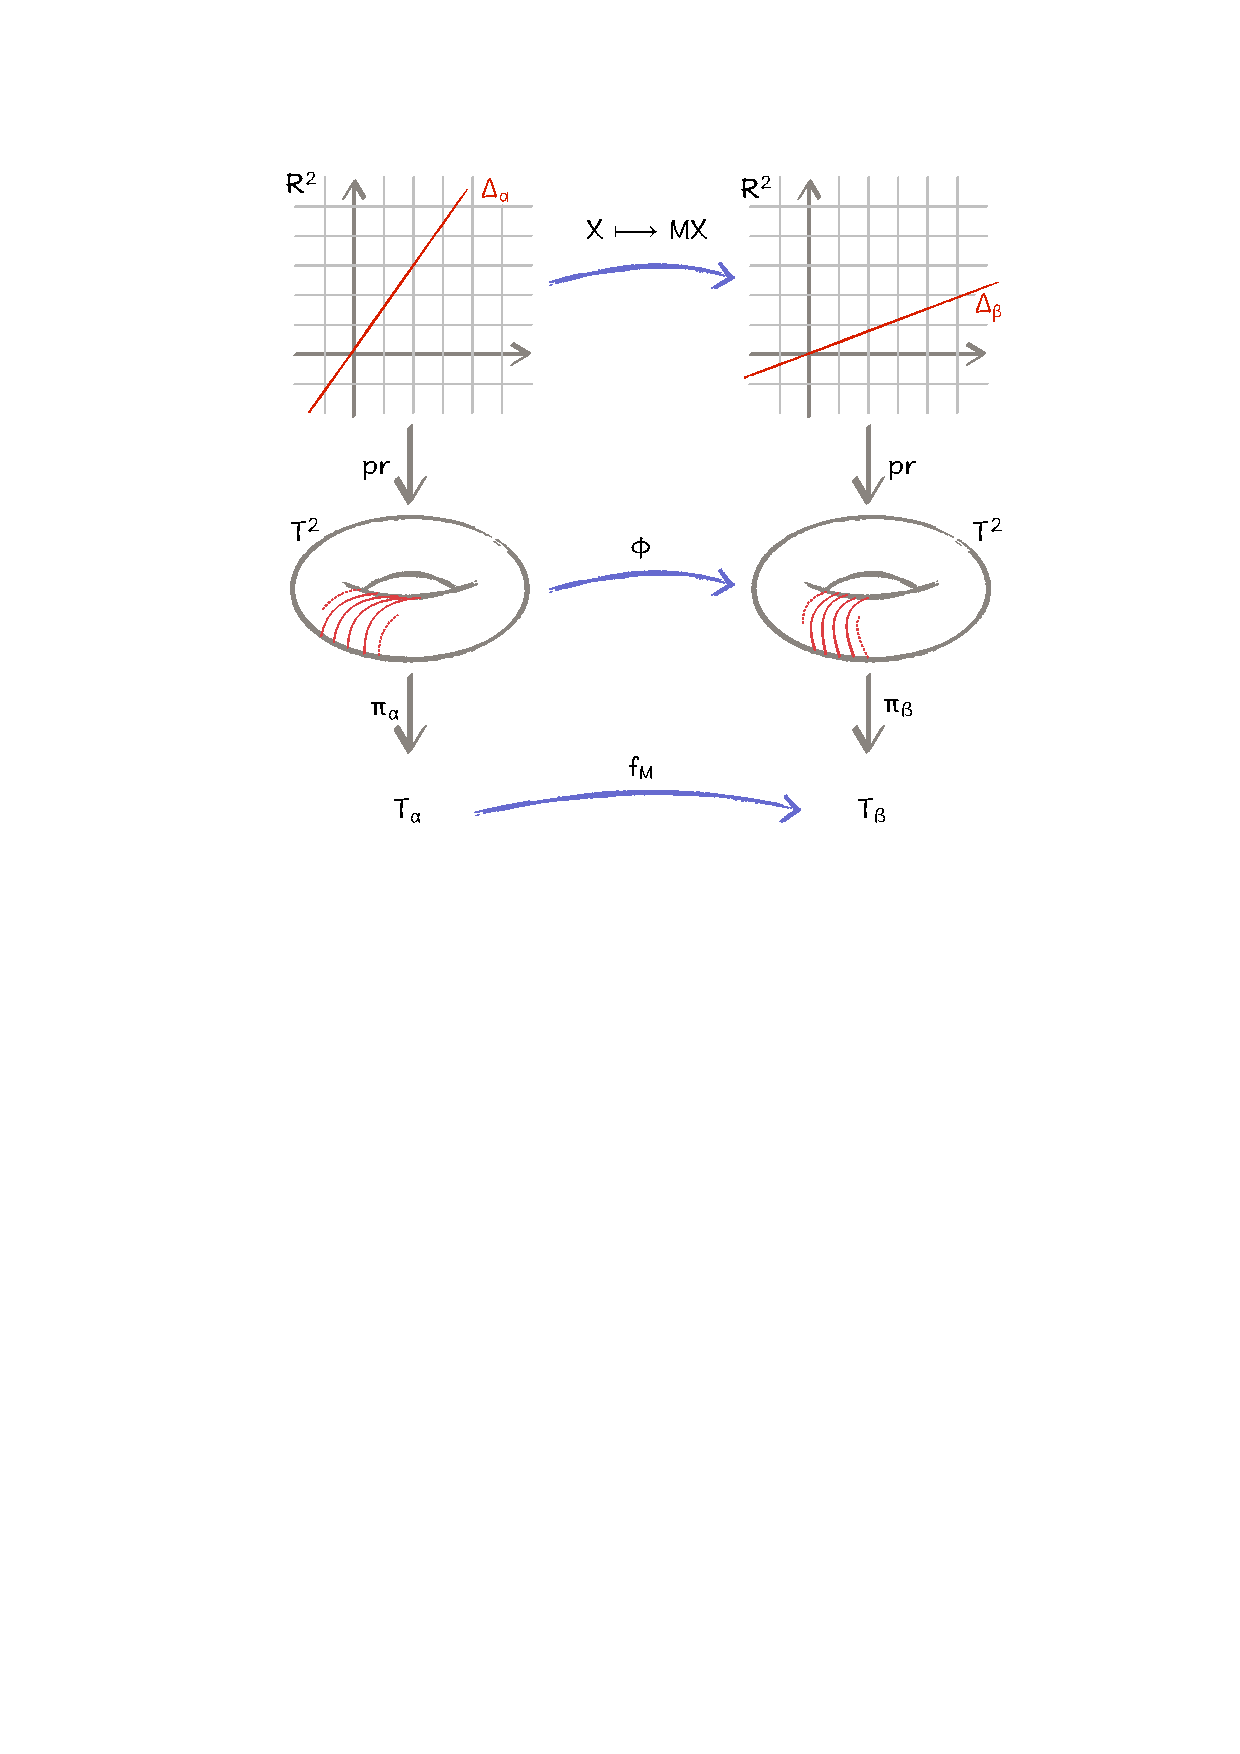
\includegraphics[width=0.65\textwidth]{Figures/T2-MDelta.pdf}
    \caption{Linear morphism from $\Torus_\alpha$ to $\Torus_\beta$.}
    \label{T2-MDelta}
  \end{figure}
  Composed with a constant map we obtain all the smooth maps from $\Torus_\alpha$ to $\Torus_\beta$,
  in additive notation:
  $$%
    f : \tau \mapsto f_M(\tau) + \nu.
    $$%
  In other words:
  
  \begin{Article}{Proposition.}
    Every smooth map $f \colon \Torus_\alpha \to \Torus_\beta$ is the projection of an affine map
    $$%
      F \colon X \to M X+ N
      \quad \text{with} \quad
      M \in \Lin(2,\ZZ)
      \quad \text{and} \quad
      N \in \RR^2.
      $$%
  \end{Article}
  
  In particular,
  the congruence modulo $\GL(2,\ZZ)$ between $\alpha$ and $\beta$,
  in case of diffeomorphism,
  is the optimum condition we can hope for a good theory of quotients.
  What is remarkable here is that this is the \smuline{sufficient and necessary condition} in the framework of diffeology.
  \smuline{Diffeology optimally discriminates the irrational tori}.
  
  Now,
  consider the set of lines in $\RR^2$,
  denoted usually by $P_2(\RR)$.
  Each line $\Delta_\alpha$ defines a torus $\Torus_\alpha$.
  
  \begin{Article}{Proposition.}
    The class of equivalent irrational tori are in bijection with the orbits of  the irrational lines by $\GL(2,\ZZ)$.
  \end{Article}
  
  Note that this proposition extends to any quotients $\Torus_\alpha = \Torus^2/\cS_\alpha$,
  even if $\alpha \in \QQ$,
  in that case $\Torus_\alpha$ is diffeomorphic to the circle $\Sph^1$.
  The rational lines are one orbit under $\GL(2,\ZZ)$.
\end{Article}

\begin{Article}{Remark: $\Cinfty(\Torus_\alpha,\Torus_\beta)$ as bimodule.}{}
  Let us come back to the lifting on $\RR$ of the smooth maps from $\Torus_\alpha$ to $\Torus_\beta$,
  \begin{center}
    \begin{tikzcd}[column sep=large, row sep=large, every label/.append style = {font = \small}]
      x \arrow[r, "F"] \arrow[d, swap, "\Class_\alpha"] &  \lambda x + \mu  \arrow[d, "\Class_\beta"]  \\
      \Class_\alpha(x) \arrow[r, swap, "f"] & \Class_\beta(\lambda x) + \Class_\beta(\mu)
    \end{tikzcd}
  \end{center}
  Since $\Torus_\beta$ is a group,
  the set $\Cinfty(\Torus_\alpha,\Torus_\beta)$ is a group for the addition.
  The mapping
  $$%
    j \colon f \mapsto (\lambda, \rho)
    \quad \text{with} \quad
    \rho = \Class_\beta(\mu),
    $$%
  is a group homomorphism.
  The map $j$ is injective and identifies
  $$%
    \Cinfty(\Torus_\alpha,\Torus_\beta) \simeq \Lambda_{\alpha\beta} \times \Torus_\beta,
    $$%
  with
  $$%
    \Lambda_{\alpha \beta} = \{ \lambda  \mid \lambda(\ZZ + \alpha \ZZ) \subset \ZZ + \beta \ZZ \}.
    $$%
  We can note here that the linear smooth maps on $\Torus_\alpha$ act on the left on $\Cinfty(\Torus_\alpha,\Torus_\beta)$,
  and the linear smooth maps on $\Torus_\beta$ act on the right.
  We can denote that by
  $$%
    \Lambda_{\alpha\alpha} \cdot \Lambda_{\alpha\beta} \cdot \Lambda_{\beta\beta} \subset \Lambda_{\alpha\beta}.
    $$%
  That would correspond to
  $$%
    x \mapsto \nu x \mapsto \lambda(\nu x) + \rho \mapsto \epsilon(\lambda(\nu x)) + \rho,
    $$%
  where $\nu(\ZZ + \alpha \ZZ) \subset \ZZ + \alpha \ZZ$ and $\epsilon(\ZZ + \beta \ZZ) \subset \ZZ + \beta \ZZ$.
  These actions are commutative and make $\Cinfty(\Torus_\alpha,\Torus_\beta)$ a bimodule.
  \uline{But this bimodule is not trivial only if $\alpha$ or $\beta$ are quadratic numbers},
  or both.
  Indeed,
  $\nu(\ZZ + \alpha \ZZ) \subset \ZZ + \alpha \ZZ$ implies there exists four integers $a,b,c,d \in \ZZ$ such that
  $$%
    \alpha = {a + b \alpha \over c + d \alpha}
    \quad \Rightarrow \quad
    d\alpha^2 + (c-b)\alpha -a =0.
    $$%
  Yet,
  still much needs to be clarified here.
\end{Article}

\begin{proof}
  We just prove that the map $j$ is injective.
  Let $\Class_\beta(\lambda x) + \rho = \Class_\beta(\lambda' x) + \rho'$,
  for $x=0$ we get $\rho = \rho'$, and then $\Class_\beta\big((\lambda - \lambda') x\big) = 0$ for all $x \in \RR$.
  That is,
  $(\lambda - \lambda') x \in \ZZ + \beta \ZZ$ for all $x \in \RR$,
  and thus $\lambda = \lambda'$.
\end{proof}

\begin{Article}{Remark: Component of $\Cinfty(\Torus_\alpha,\Torus_\beta)$.}{}
  We have seen that $\Cinfty(\Torus_\alpha,\Torus_\beta)$ is isomorphic to $\Lambda_{\alpha\beta} \times \Torus_\beta$,
  equipped with the functional diffeology the subgroup $\Lambda_{\alpha\beta} \times \{0\}$ is discrete,
  it represents the connected components,
  what we shall denote later by
  $$%
    \pi_0\big(\Cinfty(\Torus_\alpha,\Torus_\beta)\big) = \Lambda_{\alpha\beta}.
    $$%
  What we know better is the group of components of the group $\Diff(\Torus_\alpha)$.
  That is,
  the set of numbers $\lambda \in \RR$ such that:
  $$%
    \lambda (\ZZ + \alpha \ZZ) \subset \ZZ + \alpha \ZZ
    \quad \text{and} \quad
    {1 \over \lambda} (\ZZ + \alpha \ZZ) \subset \ZZ + \alpha \ZZ
    $$%
  Considering the basis $(1, \alpha)$ of the $\ZZ$-module $\ZZ + \alpha \ZZ$,
  we define $a,b,c,d$ by:
  $$%
    \lambda \times 1 = a + b \alpha
    \quad \text{and} \quad
    \lambda \times \alpha = c + d \alpha.
    $$%
  The map $F$ lifting $f$ associated with $\lambda$ for $\rho = 0$ is represented by the matrix
  $$%
    M = \Vector{a & b \\ c & d} \in \GL(2,\ZZ),
    $$%
  and it satisfies:
  \begin{equation} \tag{$\clubsuit$}
    F(x) = (a + b \alpha)x
    \quad \text{with} \quad
    \alpha = {c + d \alpha \over a + b \alpha}
    \quad \text{and} \quad
    ad - bc = \pm 1.
  \end{equation}
  As we said,
  except for the obvious solution $\lambda = 1$ which corresponds to the inversion $x \mapsto -x$,
  there are no other solutions except in the case of $\alpha$ is quadratic.
  
  Let us remark now that if two matrices $M$ and $M'$ representing $\lambda$ in $\GL(2,\ZZ)$, then they are equal.
  Indeed,
  $$%
    \lambda = \lambda' \quad \Rightarrow \quad a + b \alpha = a' + b' \alpha
    \quad \Rightarrow \quad a = a' \quad \text{and} \quad b=b'.
    $$%
  Then,
  \begin{eqnarray*}
    \alpha = {c + d \alpha \over a + b \alpha} = {c' + d' \alpha \over a' + b' \alpha}
    & \Rightarrow & c + d \alpha = c' + d' \alpha \\
    & \Rightarrow & c = c' \quad \text{and} \quad d= d'.
  \end{eqnarray*}
  Hence $M = M'$.
  
  \textbf{Proposition.}{\itshape The set of components of $\Diff(\Torus_\alpha)$ is isomorphic to the stabilizer,
  in $\GL(2,\ZZ)$,
  of the line $\Delta_\alpha$:
  $$%
    \pi_0(\Diff(\Torus_\alpha)) = \left\{ \Vector{a & b \\ c & d} \mid  \Vector{a & b \\ c & d} \Vector{1 \\ \alpha} = \lambda \Vector{1 \\ \alpha} \right\}
    $$%
  }
  According to Dirichlet's famous theorem,
  that we shall see in full generality in the next section,
  we have:
  
  \textbf{Theorem.}{\itshape The group of components of $\Diff(\Torus_\alpha)$ is isomorphic to $\{\pm 1\} \times \ZZ$ if $\alpha$ is quadratic,
  otherwise it is reduced to $\{\pm 1\}$.
  }
\end{Article}

%%%%%%%%%%%%%%%%%%%%%%%%%%%%%%%%%%%%%%%%%%%%%%%%%%%%%%%%%%
%%
%% MARK: The general codimension $1$ case
%%
%%%%%%%%%%%%%%%%%%%%%%%%%%%%%%%%%%%%%%%%%%%%%%%%%%%%%%%%%%
\section{The general codimension $1$ case}

The case presented here of an irrational hyperplane in the torus $\Torus^n$ is the result of a joint work with Gilles Lachaud,
published in 1990 \cite{IL90}. The arithmetic material for this part can be found in \cite{BC67}.

We consider the standard torus $\Torus^n = \RR^n/\ZZ^n$.

\begin{Article}{Definition.}{\itshape}
  We call \emph{irrational hyperplane} in $\RR^n$ a hyperplane $H$ that does not contain any integer points except $0$
  $$%
    H \cap \ZZ^n = \{0\}.
    $$%
  A hyperplane is directed by a linear $1$-form that is in our case normalized as follows:
  $$%
    H = \ker (w = (1\ w_2\ \dots\ w_n)) = \{x \in \RR^n \mid w(x) = \sum_{i=1}^n w_i x_i = 0 \}.
    $$%
  The fact that the hyperplane is irrational is equivalent to the property of the coefficients $w_i$ to be \smuline{independent over $\QQ$}:
  $$%
    \forall q_i \in \QQ, \quad \sum_{i = 1}^n w_i q_i = 0 \quad \Rightarrow \quad q_i = 0, \forall i.
    $$%
  Let us denote by $\cS_H \subset \Torus^n$ the image of $H$ by the canonical projection $\pi \colon \RR^n \to \Torus^n$.
  Here again the map $\pi \restriction H$ is an induction.
  
  We define the \emph{irrational torus associated with $H$} as the quotient space
  $$%
    T_H = \Torus^n/\cS_H,
    $$%
  which is also an Abelian group.
\end{Article}

\begin{Article}{Proposition.}{\itshape}
  The space $T_H$ is diffeomorphic to the quotient:
  $$%
    T_H \simeq \RR/w(\ZZ^n).
    $$%
  where
  $$%
    w(\ZZ^n) = \{n_1 + \sum_{i=2}^n w_i n_i \mid n_i \in \ZZ \}
    $$%
  is a subgroup of $(\RR,+)$.
\end{Article}

\begin{Article}{The group $\Diff(T_H)$.}{\itshape}
  The group of diffeomorphisms of the irrational torus $T_H$ is given by
  $$%
    \Diff(T_H) \simeq \Lambda_w \times T_H.
    $$%
  with $\Lambda_w$ its group of components $\pi_0(\Diff(T_H))$:
  $$%
    \Lambda_w = \{ \lambda \in \RR \mid \lambda \cM_w = \cM_w \}
    \quad \text{with} \quad
    \cM_w = w(\ZZ^n).
    $$%
\end{Article}

\begin{proof}
  The situation for the diffeomorphisms of the torus $T_H$ is identical to the case of $\Torus_\alpha$.
  They are the projections $f$ of the affine maps
  $$%
    F \colon x \mapsto \lambda x + \mu,
    $$%
  such that,
  for all $k \in \ZZ^n$ there exists a unique $k' \in \ZZ^n$ with $F(w(k)) = w(k')$.
  In other words,
  $$%
    \lambda w(\ZZ^n) \subset w(\ZZ^n).
    $$%
  The map $f \in \Diff(T_H)$ is then defined by
  $$%
    f \circ \Class_w(x) = \Class_w(F(x)).
    $$%
  On $T_H$,
  $f$ is the composite of the linear part
  $$%
    \underline \lambda \colon \Class_w(x) \mapsto \Class_w(\lambda x)
    $$%
  by some translation
  $$%
    \bmt_\rho \colon \Class(x) \mapsto \Class_w(x) + \rho
    \quad \text{with} \quad
    \rho = \Class_w(\mu).
    $$%
  We can focus on the linear parts of the diffeomorphisms of $T_H$,
  which makes the discrete part of $\Diff(T_H)$.
  
  Consider now the inverse diffeomorphism $(\underline{\lambda})^{-1}$,
  it can be lifted to $\RR^n$ by $\underline{\lambda'}$,
  with
  $$%
    \underline{\lambda} \circ \Class_w = \Class_w \circ \underline{\lambda}
    \quad \text{and} \quad
    \Class_w \circ \underline{\lambda'} = (\underline{\lambda})^{-1} \circ \Class_w,
    $$%
  where $\underline{\lambda}$ on $\RR$ is just the multiplication by $\lambda$.
  We get
  $$%
    \Class_w \circ \underline{\lambda'} \circ \underline{\lambda} = \Class_w,
    $$%
  which gives first $\lambda'\lambda x = x + w(k)$,
  with $k \in \ZZ^n$,
  and then $k=0$ for $x=0$.
  Therefore
  $$%
    \lambda' = {1 \over \lambda}.
    $$%
  Thus,
  $$%
    {1 \over \lambda} w(\ZZ^n) \subset w(\ZZ^n)
    \quad \Rightarrow \quad
    \lambda \times {1 \over \lambda} w(\ZZ^n) \subset \lambda w(\ZZ^n).
    $$%
  Therefore,
  $\lambda w(\ZZ^n) \subset w(\ZZ^n)$ and $w(\ZZ^n) \subset \lambda w(\ZZ^n)$,
  that is,
  $$%
    \lambda w(\ZZ^n) = w(\ZZ^n).
    $$%
  We get then the discrete part of $\Diff(T_H)$
  $$%
    \Lambda_w = \{ \lambda \in \RR \mid \lambda \cM_w = \cM_w \},
    $$%
  such that $\Diff(T_H) \simeq \Lambda_w \times T_H$.
\end{proof}

In order to understand the group of components $\Lambda_w$ we will introduce the $\QQ$-vector space:
$$%
  E_w = w(\QQ^n) = \bigg\{ q_1 + \sum_{i=2}^n q_i w_i \mid q_i \in \QQ\bigg\}.
  $$%

\begin{Article}{The Algebraic Field $K_w$.}{\itshape}
  The set of numbers
  $$%
    K_w = \{ \lambda \in \RR \mid \lambda E_w \subset E_w \}
    $$%
  is an \emph{algebraic number field},
  a finite extension of $\QQ$,
  whose dimension $d$ on $\QQ$ divides $n$,
  and $E_w$ is a $K_w$-vector space of dimension $n/d$.
  That is,
  $K_w$ is a field $\QQ(\theta)$ where $\theta$ is a solution of some polynomial with integer coefficients.
\end{Article}

\begin{proof}
  It is enough to prove that if $k\in K_w$  and $k\neq 0$,
  then $1/k\in K$.
  The multiplication by $k$ is a linear map in $E_w$ whose kernel is $\{0\}$,
  then it is injective.
  Since $E_w$ is finite dimensional,
  it is surjective:
  for all $y \in E_w$ there exists $x \in E$ such that $kx=y$,
  that is,
  $x = y/k$.
  the number $1/k$ stabilizes $E_w$.
  On the other hand,
  $K_w$ is a subalgebra of $\Lin(E)$,
  hence of finite dimension on $\QQ$.
  Since $\QQ \subset K_w$,
  $K_w$ is a finite extension of $\QQ$.
  Moreover,
  the space $E_w$ is naturally a $K_w$-module,
  it is then a $K_w$-vector space.
  We get then  $\dim_{\QQ} E_w = \dim_{\QQ} K_w \times \dim_{K_w} E_w$.
\end{proof}

Let us consider now a lattice $\cM_w \subset E_w$,
that is,
an additive subgroup of $E_w$ such that $\cM_w \otimes \QQ = E_w$.
Its ring of stabilizers:
$$%
  A_w = \{\lambda \in \RR \mid \lambda \cM_w \subset \cM_w \}
  $$%
is a subring of the field $K_w$.

Let us recall what is  an \emph{order} in the sense of ring theory (op.\,cit.).

\begin{Article}{Order of a ring.}{\itshape}
  Let $K$ be a ring that is a \uline{finite-dimensional algebra over the field $\QQ$}.
  Let $A \subset K$ be a subring.
  We say that $A$ is an \emph{order} of $K$ if
  \begin{enumerate}
    \item $A$ is a $\ZZ$-lattice in $K$,
    \item $A$ spans $K$ over $\QQ$.
  \end{enumerate}
\end{Article}

Then,

\begin{Article}{The Order $\cM_w$.}{}
  Let $E \subset \RR$ be a finite dimensional $\QQ$-vector subspace,
  and $\cM \subset E$ be a $\ZZ$-lattice.
  The ring $A$ of stabilizers of $\cM$
  $$%
    A  = \{ \lambda \in \RR \mid \lambda \cM \subset \cM \},
    $$%
  is an order of the ring $K$ of the stabilizer of $E$ in $\RR$
  $$%
    K = \{ \lambda \in \RR \mid \lambda E \subset E \}.
    $$%
  In other words:
  $$%
    E = \cM \otimes \QQ \quad \Rightarrow \quad K = A \otimes \QQ.
    $$%
\end{Article}

\begin{proof}
  We want to prove that $K = A \otimes \QQ$.
  Let $w=(w_1,\ldots,w_n)$ be a $\ZZ$-basis of $\cM$,
  {\itshape i.e.}\/ a $\QQ$-basis of $E = \cM \otimes \QQ$ such that $w(\ZZ^n)=\cM$.
  Let $\lambda \in K$ and $\Lambda$ be the matrix representing $\underline\lambda$,
  the multiplication by $\lambda \in K$,
  in the basis $w$.
  The matrix $\Lambda$ can be written $\Lambda = \Lambda'/\ell$,
  where $\ell \in \ZZ$ is the least common multiple of the denominators of the elements of $\Lambda$,
  and  $\Lambda' \in \Lin(\ZZ^n)$.
  For all $m \in \cM$ we have then $\ell \lambda m \in \cM$,
  that is,
  $(\ell\lambda) \cM \subset \cM$.
  Therefore,
  $\ell \lambda \in A$,
  or again $\lambda \in A \otimes \QQ$.
\end{proof}

So,
coming back to $A_w$ and $K_w$,
$A_w$ is an order of $K_w$.
Now we are not just interested in $A_w$ but in its invertible elements.
That is,
\begin{align*}
  \Lambda_w & = \{ \lambda \in \RR \mid \lambda \cM \subset \cM \text{ and } {1 \over \lambda} \cM \subset \cM \}, \\
  & = \{ \lambda \in A_w \mid \lambda^{-1} \in A_w \}.
\end{align*}

\begin{Article}{The Group $\Lambda_w$.}{}
  The group $\Lambda_w$ of components of $\Diff(T_H))$ is the group of invertible elements of the ring $A_w$,
  that is,
  its group of units (op.\,cit.).
  Since $A_w$ is an order of the algebraic field $K_w$,
  its group of units is given by the \emph{Dirichlet's unit theorem}.%
  \footnote{\url{https://www.wikipedia.org/en/Dirichlet's_unit_theorem}}
  In our case:
  $$%
    \Lambda_w \simeq {\pm1} \times \ZZ^{r+s-1},
    $$%
  where $r$ is the number of real places of the field $K_w$ and $2s$ the number of complex places.
  In other words,
  $K_w = \QQ(\theta)$ where $\theta$ is a solution of a polynomial $P$ with integer coefficients.
  The degree $d$ of $K_w$ divides $n$,
  thus $d = r + 2s$ and $n = \ell d$.
  
  \Note In particular,
  for $n = 2$ there are two cases,
  either $d = 0$ and $\Lambda_w = \{\pm1\}$,
  or $d = 2$ and $\Lambda_w = \{\pm1\} \times \ZZ$.
\end{Article}

\begin{Article}{Example.}{}
  For the quotient of a $2$-torus there is,
  as we have seen,
  only one possibility:
  if we have one real root of the characteristic polynomial,
  we have two and then $\pi_0(\Diff(\Torus/H) = \{\pm 1\} \times \ZZ$.
  For a $3$-torus we have two possibilities either our characteristic polynomial has one real root or three,
  illustrated in Figure \ref{Algebraic-fields}.
  
  In the first case the order is generated by one generator $\chi$,
  and $\pi_0(\Diff(\Torus/H) = \{\pm 1\} \times \ZZ$.
  $$%
    w = (1\ \sqrt[3]{2}), \quad  \chi = \sqrt[3]{2} -1.
    $$%
  In the second case the order of $K_w$ has two generators $\chi$ and $\chi'$,
  and $\pi_0(\Diff(\Torus/H') = \{\pm 1\} \times \ZZ^2$.
  $$%
    w = (1 \ \rho \ \rho^2),
    \text{ with } \
    \rho = 2\cos\big({2\pi \over 9}\big),
    \ \chi = \rho,
    \text{ and } \
    \chi' = {1 \over 1-\rho}.
    $$%
  
  \smallskip
  \begin{figure}[hb]
    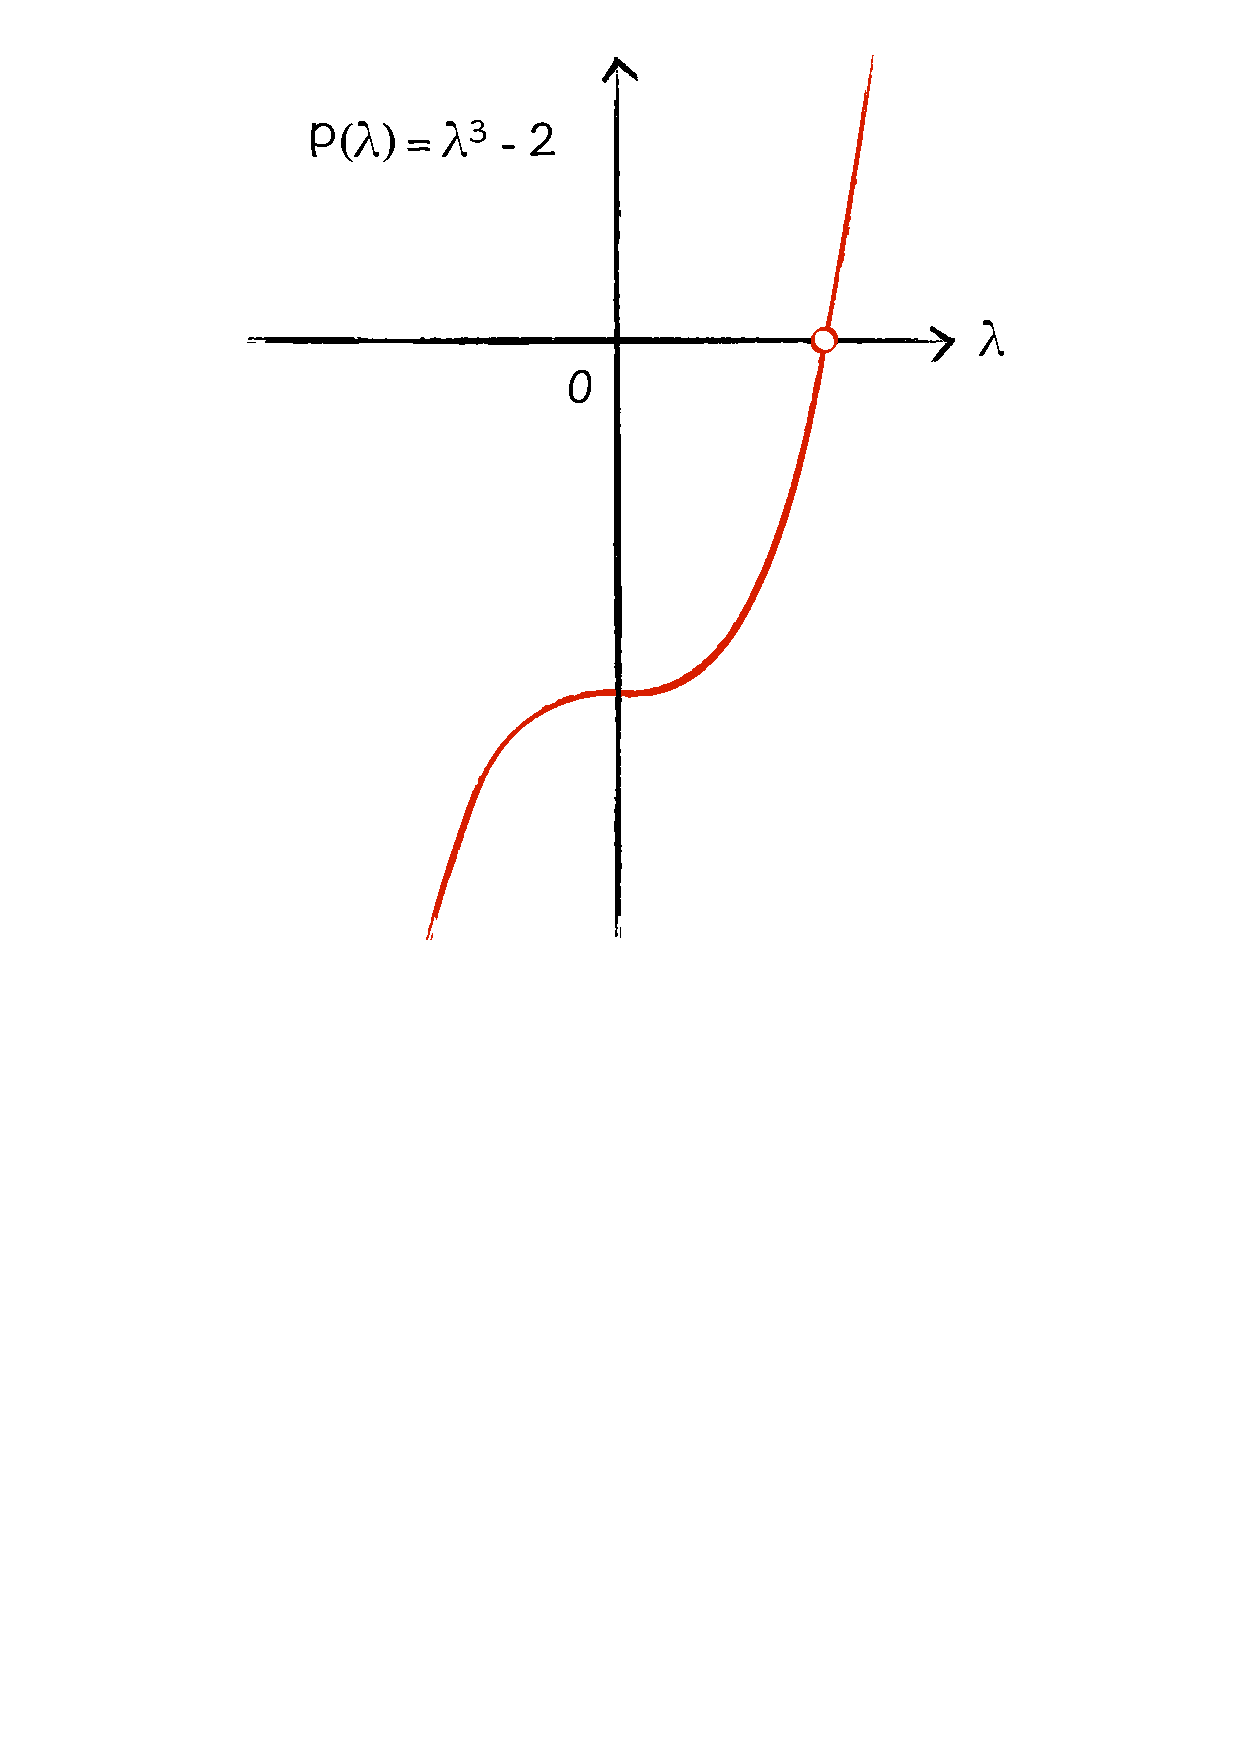
\includegraphics[width=.33\textwidth]{Figures/Algebraic-field-1.pdf}
    \quad
    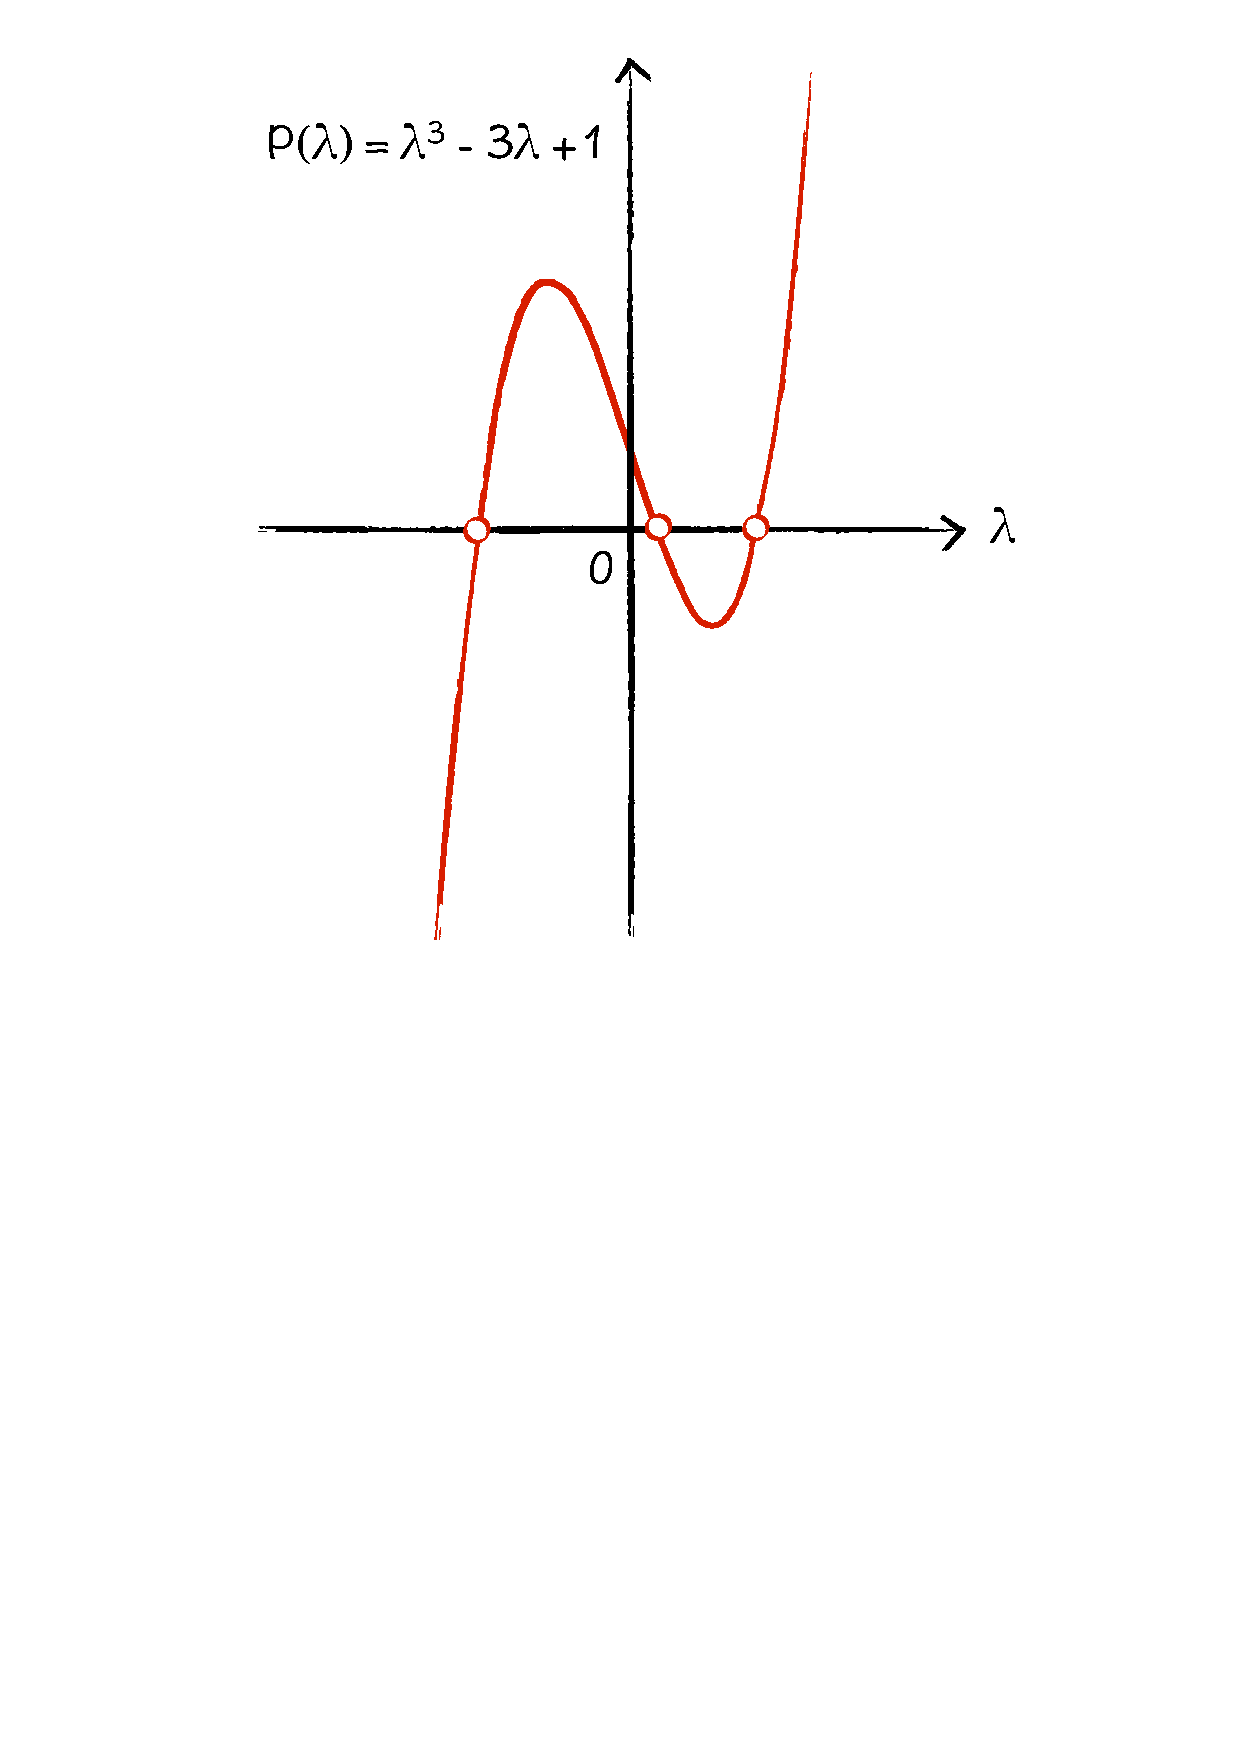
\includegraphics[width=.4\textwidth]{Figures/Algebraic-field-2.pdf}
    \caption{The two examples for $\Torus^3$.}
    \label{Algebraic-fields}
  \end{figure}
  
\end{Article}
